%%%%%%%%%%%%%%%%%%%%%%%%%%%%%%%%%%%%%%%%%
% Uppsala University Assignment Title Page 
% LaTeX Template
% Version 1.0 (27/12/12)
%
% This template has been downloaded from:
% http://www.LaTeXTemplates.com
%
% Original author:
% WikiBooks (http://en.wikibooks.org/wiki/LaTeX/Title_Creation)
% Modified by Elsa Slattegard to fit Uppsala university
% License:
% CC BY-NC-SA 3.0 (http://creativecommons.org/licenses/by-nc-sa/3.0/)

%\title{Title page with logo}
%----------------------------------------------------------------------------------------
%	PACKAGES AND OTHER DOCUMENT CONFIGURATIONS
%----------------------------------------------------------------------------------------

\documentclass[12pt]{article}

\usepackage{tikz,lipsum,lmodern}
\usepackage[most]{tcolorbox}

\usepackage[utf8]{inputenc}
\usepackage[greek,english]{babel}
\usepackage{alphabeta}
\usepackage{amsmath}
\usepackage{gfsartemisia}
\usepackage{graphicx}

\usepackage{float}
\usepackage[colorinlistoftodos]{todonotes}
\usepackage{tabularx}
\usepackage[myheadings]{fullpage}
\usepackage{enumitem}
\PassOptionsToPackage{hyphens}{url}\usepackage{hyperref}
\usepackage{tikz}
\usepackage[nottoc]{tocbibind} %Adds "References" to the table of contents
\usepackage{xcolor} % to access the named colour LightGray
\definecolor{LightGray}{gray}{0.9}

\usepackage{caption}
\usepackage{subcaption}

\usepackage[edges]{forest}
\definecolor{folderbg}{RGB}{124,166,198}
\definecolor{folderborder}{RGB}{110,144,169}

%================ file tree =====================%
\usepackage[edges]{forest}
\definecolor{folderbg}{RGB}{124,166,198}
\definecolor{folderborder}{RGB}{110,144,169}
\newlength\Size
\setlength\Size{4pt}
\tikzset{%
	folder/.pic={%
		\filldraw [draw=folderborder, top color=folderbg!50, bottom color=folderbg] (-1.05*\Size,0.2\Size+5pt) rectangle ++(.75*\Size,-0.2\Size-5pt);
		\filldraw [draw=folderborder, top color=folderbg!50, bottom color=folderbg] (-1.15*\Size,-\Size) rectangle (1.15*\Size,\Size);
	},
	file/.pic={%
		\filldraw [draw=folderborder, top color=folderbg!5, bottom color=folderbg!10] (-\Size,.4*\Size+5pt) coordinate (a) |- (\Size,-1.2*\Size) coordinate (b) -- ++(0,1.6*\Size) coordinate (c) -- ++(-5pt,5pt) coordinate (d) -- cycle (d) |- (c) ;
	},
}
\forestset{%
	declare autowrapped toks={pic me}{},
	pic dir tree/.style={%
		for tree={%
			folder,
			font=\ttfamily,
			grow'=0,
		},
		before typesetting nodes={%
			for tree={%
				edge label+/.option={pic me},
			},
		},
	},
	pic me set/.code n args=2{%
		\forestset{%
			#1/.style={%
				inner xsep=2\Size,
				pic me={pic {#2}},
			}
		}
	},
	pic me set={directory}{folder},
	pic me set={file}{file},
}

%=================================================%


\usepackage{tabto}
\usepackage{minted}


\hyphenpenalty=10000


\usepackage{geometry}
\geometry{
	a4paper,
	total={170mm,257mm},
	left=20mm,
	top=20mm,
}


\addto\captionsenglish{% Replace "english" with the language you use
	\renewcommand{\contentsname}%
	{Περιεχόμενα}%
}

\addto\captionsenglish{
	\renewcommand{\partname}{}
}
\renewcommand{\thepart}{}

\makeatletter
\renewcommand{\fnum@figure}{Εικόνα \thefigure}
\makeatother


\renewcommand{\H}{\textlozenge}

%=====fonts==========%
%\usepackage{libertine}


%====================%





%=============header + footer ======================%
%

\usepackage{fancyhdr}

\pagestyle{fancy}
\fancyhf{}
\rhead{Σύγχρονα θέματα Τεχνολογίας Λογισμικού 
\includegraphics[width=0.7cm]{UNIPI_(logo).png}}
\lhead{Πανεπιστήμιο Πειραιώς \\ Τμήμα Πληροφορικής}
\cfoot{Σελίδα \thepage}

% 

%\setlength\headheight{47pt}
%=====================================================%



%\setcounter{secnumdepth}{0} % sections are level 1

\begin{document}
	
	\begin{titlepage}
		
		\newcommand{\HRule}{\rule{\linewidth}{0.5mm}} % Defines a new command for the horizontal lines, change thickness here
		
		\center % Center everything on the page
		
		%----------------------------------------------------------------------------------------
		%	HEADING SECTIONS
		%----------------------------------------------------------------------------------------
		
		\textsc{\LARGE Πανεπιστήμιο Πειραιώς}\\[1.5cm] % Name of your university/college
		
\includegraphics[scale=0.6]{UNIPI_(logo).png}\\[1cm] % Include a department/university logo - this will require the graphicx package
		\textsc{\Large Τμήμα Πληροφορικής}\\[0.5cm] % Major heading such as course name
		\textsc{\large Σύγχρονα θέματα Τεχνολογίας Λογισμικού - Λογισμικό για κινητές συσκευές}\\[0.5cm] % Minor heading such as course title
		
		%----------------------------------------------------------------------------------------
		%	TITLE SECTION
		%----------------------------------------------------------------------------------------
		
		\HRule \\[0.4cm]
		{ \Large \bfseries Αριστοτέλης Ματακιάς - Α.Μ: Π19100}\\[0.4cm] % Title of your document
		{ \Large \bfseries Βασίλη Γκιάτα - Α.Μ. Π19036}\\[0.4cm] % Title of your document
		\HRule \\[1.5cm]
		
		%----------------------------------------------------------------------------------------
		%	AUTHOR SECTION
		%----------------------------------------------------------------------------------------
		%
		
		\textsc{\Large Εργασία στο μοντέλο Model View Controller \\[0.4cm] Τεχνικό Εγχειρίδιο} % Minor heading such as course title
		
		% If you don't want a supervisor, uncomment the two lines below and remove the section above
		%\Large \emph{Author:}\\
		%John \textsc{Smith}\\[3cm] % Your name
		
		%----------------------------------------------------------------------------------------
		%	DATE SECTION
		%----------------------------------------------------------------------------------------
		
		
		
		\vfill % Fill the rest of the page with whitespace
		
	\end{titlepage}
	
	%\selectlanguage{greek}
	\tableofcontents
	%\selectlanguage{english}
	
	 \newpage
	
%	 \section{Εισαγωγή}
%	 Στο παρόν έγγραφο περιλαμβάνεται η τεχνική αναφορά για το project με τίτλο \textbf{UniveristyApp} (ASP.NET Core Web Application). Η γλώσσα προγραμματισμού είναι C\# και η βάση δεδομένων δημιουργήθηκε με το εργαλείο Microsoft Sql Server 2022.
%	 
%	 Στις ενότητες που ακολουθούν αναλύονται αρχικά τα ζητούμενα της εργασίες και στην συνέχεια οι λεπτομέρειες υλοποίησης όπου αναλύονται τα επίπεδα \textbf{Model}, \textbf{View} και \textbf{Controller}.
%	
%	 \newpage
	
	\section{Ζητούμενα}
	
	Να αναπτύξετε μια διαδικτυακή εφαρμογή βαθμολογίου για τους φοιτητές του πανεπιστημίου. Η εφαρμογή θα περιλαμβάνει διάφορες κατηγορίες χρηστών όπως \textbf{φοιτητές}, \textbf{καθηγητές} και \textbf{γραμματειακό προσωπικό}. Για παράδειγμα, ένας καθηγητής μπορεί να καταχωρήσει τη βαθμολογία για κάθε φοιτητή και για κάθε μάθημα που διδάσκει (τελικό βαθμό ή/και επιμέρους βαθμούς του μαθήματος όπως βαθμοί από ασκήσεις, εργασίες, γραπτό διαγώνισμα), ενώ κάθε φοιτητής μπορεί να έχει πρόσβαση στο λογαριασμό του ώστε να δει τα αποτελέσματα της βαθμολογίας του.
		
	Όλοι οι Χρήστες θα μπορούν να κάνουν Login μέσω μιας Φόρμας Login (η επιτυχής σύνδεση θα ανακατευθύνει τον χρήστη στην index σελίδα).
	
	\begin{itemize}
		
		\item Για τους Φοιτητές:
		\begin{itemize}
			\item[$\blacksquare$] Προβολή βαθμολογίας ανά μάθημα.
			\item[$\blacksquare$] Προβολή βαθμολογίας ανά εξάμηνο.
			\item[$\blacksquare$] Προβολή συνολικής βαθμολογίας (για όλα τα μαθήματα που έχει εξεταστεί).
		\end{itemize}
	
		\item Για τους Καθηγητές:
		\begin{itemize}
			\item[$\blacksquare$] Προβολή λίστας βαθμολογίας ανά μάθημα (για ήδη βαθμολογημένα μαθήματα).
			\item[$\blacksquare$] Καταχώρηση βαθμολογίας ανά μάθημα (για μη βαθμολογημένα μαθήματα).
		\end{itemize}
	
		\item Για τις Γραμματείες:
		\begin{itemize}
			\item[$\blacksquare$] Καταχώρηση Μαθημάτων, Καθηγητών, Φοιτητών.
			\item[$\blacksquare$] Προβολή μαθημάτων (τίτλος μαθήματος, εξάμηνο, υπεύθυνος Καθηγητής).
			\item[$\blacksquare$] Ανάθεση μαθήματος σε Καθηγητή.
			\item[$\blacksquare$] Δήλωση μαθήματος σε Φοιτητή.
		\end{itemize}
	
	\end{itemize}
	
	\newpage
	\section{Επίπεδο Model}
	Η υλοποίηση της εφαρμογής ξεκίνησε αρχικά από την δημιουργία της βάσης δεδομένων. Παρακάτω δίνεται το σχεσιακό σχήμα της βάσης.
	
	\begin{figure}[H]
		\centering
		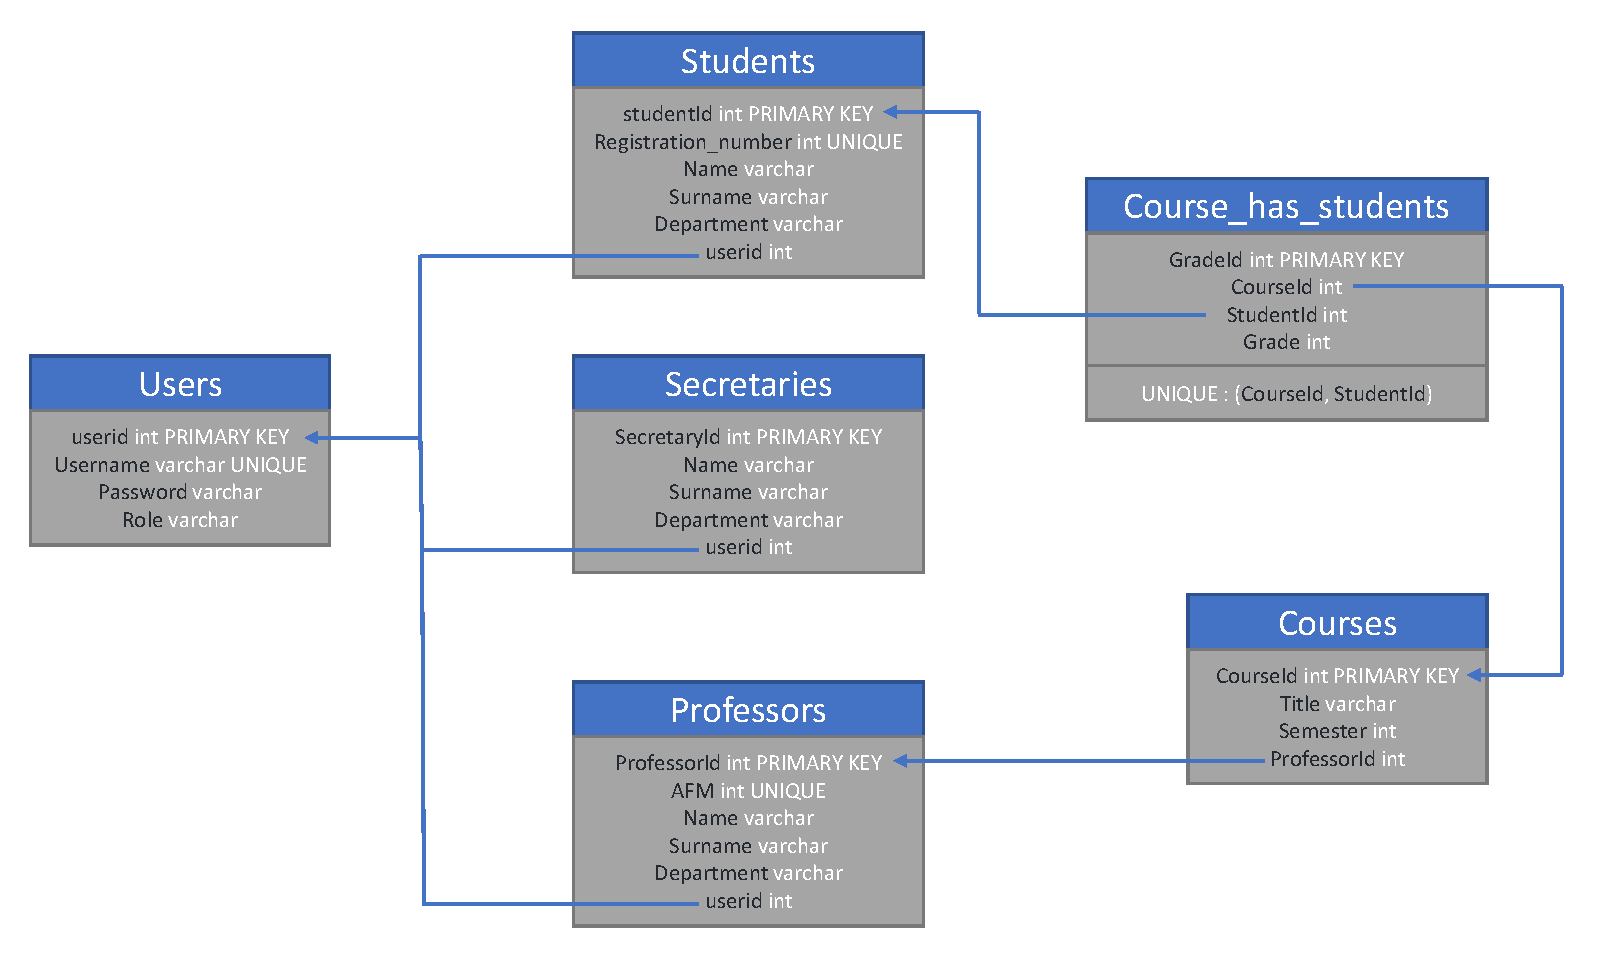
\includegraphics[width=0.85\textwidth]{table.pdf}
		\caption{}
		\label{fig:bex}
	\end{figure}
	
	Αρχικά υπάρχει ο πίνακας \textbf{Users} στον οποίο περιλαμβάνονται οι κωδικοί πρόσβασης (username και password) όλων των χρηστών της εφαρμογής. Το πεδίο UserID είναι απλώς ένας κωδικός ξεχωριστός για κάθε χρήστη και το πεδίο Role δηλώνει τον τύπο του χρήστη. Στην εφαρμογή υπάρχουν 3 βασικοί τύποι χρηστών: \textbf{Students (Φοιτητές)}, \textbf{Professors (Καθηγητές)} και \textbf{Secretaries (Γραμματείες)}. Υπάρχουν οι 3 αντίστοιχοι πίνακες οι οποίοι συνδέονται με τον πίνακα \textbf{Users} μέσω του ξένου κλειδιού (foreign key) UserID. Ο πίνακας Users θα μπορούσε να παραληφθεί αλλά επιτρέπει την εύκολη υλοποίηση του \textbf{Session Management} που θα αναλυθεί σε επόμενη ενότητα.
	
	Στη συνέχεια υπάρχει ο πίνακας \textbf{Courses} όπως δηλώνει το όνομά του περιέχει τα Μαθήματα. Κάθε μάθημα ανατίθεται σε έναν καθηγητή αποκλειστικά, γι' αυτό υπάρχει το πεδίο ProfessorId το οποίο είναι foreign key και δείχνει στο PK του πίνακα \textbf{Professors}.
	
	Ο πίνακας \textbf{Course\_has\_students} συνδέει τις εγγραφές των πινάκων \textbf{Students} και \textbf{Courses}. Περιέχει τα πεδία StudentId και CourseId τα οποία είναι foreign keys και στα PK των πινάκων \textbf{Students} και \textbf{Courses} αντίστοιχα. Επιπλέον ορίζεται ως unique το ζευγάρι των πεδίων StudentId και CourseId. Αυτό γίνεται διότι μπορεί ένας φοιτητής να έχει πολλές εγγραφές στον πίνακα \textbf{Course\_has\_students}, άρα το StudentId θα επαναλαμβάνεται, και αντίστοιχα πολλοί φοιτητές θα έχουν το ίδιο μάθημα άρα το CourseId θα επαναλαμβάνεται. Δεν πρόκειται όμως στον πίνακα \textbf{Course\_has\_students} να εισαχθεί ο ίδιος φοιτητής με το ίδιο μάθημα πάνω από μία φορά, γι' αυτό ορίζεται ο αντίστοιχος περιορισμός 2 πεδίων.
	
	Σε όλους τους πίνακες έχει οριστεί ένα Id σαν PK. Αυτό έγινε καθώς το scaffolding του Visual Studio 2022 αναγνωρίζει καλύτερα τις σχέσεις μεταξύ των πινάκων. Θεωρούμε πως σε κάθε πίνακα το Id είναι ένας αύξοντας αριθμός (AUTO INCREMENT). Οι κλάσεις των μοντέλων που προέκυψαν περιέχονται στον φάκελο Models ο οποίος έχει την παρακάτω αρχειοθέτηση:
	
\begin{figure}[H]
	\centering
	\begin{forest}
		pic dir tree,
		where level=0{}{% folder icons by default; override using file for file icons
			directory,
		},
		[Models
		[Metadata
		[CourseMetadata.cs, file
		]
		[ProfessorMetadata.cs, file
		]
		[StudentMetadata.cs, file
		]
		]
		[Course.cs, file
		]
		[CourseHasStudent.cs, file
		]
		[ErrorViewModel.cs, file
		]
		[PatialClasses.cs, file
		]
		[Professor.cs, file
		]		
		[Secretary.cs, file
		]
		[Student.cs, file
		]
		[UniveristyDBContext.cs, file
		]
		[User.cs, file
		]	
		]
	\end{forest}
	\caption{Αρχειοθέτηση του φακέλου Models}
\end{figure}
	
	Έχουν προστεθεί και Metadata κλάσεις κυρίως για την αλλαγή DisplayNames πεδίων και τη δημιουργεία computed πεδίων (όπως Fullname).
		
	\section{Επίπεδο View και Controller}
	
	\subsection{Session Management}
	Στην εκφώνηση της εργασίας αναφέρεται ότι η υλοποίηση Session Management δεν περιλαμβάνεται στα ζητούμενα. Ωστόσο αποφασίστηκε στα πλαίσια της εργασίας να συμπεριληφθεί η διαχείριση Συνόδου μέσω μίας απλής υλοποίησης. Πιο συγκεκριμένα δεν χρησιμοποιήθηκε το Microsoft Identity Platform που παρέχεται από το Visual Studio 2022 αλλά ένα custom Session management μέσω μεθόδων που περιέχονται ήδη στο MVC project.
	
	Για να γίνει πιο κατανοητή η διαδικασία θα ξεκινήσουμε με ένα παράδειγμα. Παρακάτω δίνεται μια C\# εντολή στην οποία δημιουργείται στο session ένα πεδίο string με όνομα username και περιεχόμενο 'user1'

\begin{minted}
[
frame=lines,
framesep=2mm,
baselinestretch=1.2,
bgcolor=LightGray,
fontsize=\footnotesize
]{csh}
HttpContext.Session.SetString("username", "user1");
\end{minted}

Εφόσον η εντολή αυτή εκτελεστεί, μπορούμε στη συνέχεια να ανακτήσουμε το περιεχόμενο του πεδίου username από το session με την παρακάτω εντολή:

\begin{minted}
[
frame=lines,
framesep=2mm,
baselinestretch=1.2,
bgcolor=LightGray,
fontsize=\footnotesize
]{csh}
HttpContext.Session.GetString("username")
\end{minted}

Η εντολή αυτή επιστρέφει ένα string και είναι το περιεχόμενο του πεδίου username. Πάνω σε αυτές τις εντολές βασίζεται η διαχείριση συνόδου της εφαρμογής.

Η είσοδος του χρήστη πραγματοποιείται μέσω του View \textbf{Login.cshmtl} το οποίο είναι προσβάσιμο από την αρχική σελίδα (index) του HomeController (ο οποίς είναι και ο default controller). Σε αυτό το View ο χρήστης δίνει το Username και το Password του και εκτελείται η παρακάτω Action Method.

\begin{minted}
	[
	frame=lines,
	framesep=2mm,
	baselinestretch=1.2,
	bgcolor=LightGray,
	fontsize=\footnotesize
	]{csh}
[HttpPost]
public ActionResult Login(User user)
{
	_context = new UniversityDBContext();
	var obj = _context.Users.Where(a => a.Username.Equals(user.Username) 
		&& a.Password.Equals(user.Password)).FirstOrDefault();
	if (obj != null)
	{
		HttpContext.Session.SetString("username", obj.Username.ToString());
		HttpContext.Session.SetString("userid", obj.Userid.ToString());
		HttpContext.Session.SetString("role",obj.Role.ToString());
		
		return RedirectToAction("Index", obj.Role);
	}	
	return RedirectToAction("Login");
}
\end{minted}
Μέσω ενός Post request στέλνεται στον Server ένα αντικείμενο τύπου User (περιέχει μόνο τα πεδία Username και Password - τα υπόλοιπα είναι \textbf{null}) και γίνεται έλεγχος αν υπάρχει στην βάση User με τα δοσμένα credentials. Αν δεν βρεθεί χρήστης, γίνεται Redirection στην Log in σελίδα. Αντίθετα, αν βρεθεί το αντίστοιχο User object, δημιουργούνται 3 πεδία στο Session:

\begin{itemize}
	\item Πεδίο \textbf{username} το οποίο περιέχει το Username του αντικειμένου User
	\item Πεδίο \textbf{userid} το οποίο περιέχει το UserId του αντικειμένου User
	\item Πεδίο \textbf{role} το οποίο περιέχει το Role του αντικειμένου User
\end{itemize} 

Οι πληροφορίες αυτών των πεδίων είναι απαραίτητες, καθώς χάρις αυτές θα καθορίζεται σε ποιες λειτουργίες της εφαρμογής θα έχει πρόσβαση ο χρήστης που συνδέθηκε. Για παράδειγμα ένας Καθηγητής μπορεί να δει μόνο τα δικά του μαθήματα και τις αντίστοιχες βαθμολογίες του και όχι μαθήματα άλλων καθηγητών. Αντίστοιχα δεν επιτρέπεται ένας Φοιτητής ή ένας Καθηγητής να έχει πρόσβαση σε σελίδες της Γραμματείας. Πριν εξηγήσουμε πώς θα γίνονται αυτοί οι έλεγχοι πρέπει να αναφέρουμε την γενική δομή των Controller της εφαρμογής. Όπως φαίνεται στην παραπάνω συνάρτηση \textbf{Login} μετά τον ορισμό των πεδίων του Session ο χρήστης ανακατευθύνεται στην Index σελίδα του controller με όνομα το περιεχόμενο του πεδίου \textbf{user.Role}. Από σύμβαση της Βάσης Δεδομένων Users που είναι οι Φοιτητές, οι Καθηγητές και οι Γραμματείες περιέχουν στο πεδίο Role την λέξη 'Students', 'Professors' και 'Secretaries' αντίστοιχα. Οι τρεις αυτοί όροι αντιστοιχοούν στους Controllers της εφαρμογής: \textbf{StudentsController}, \textbf{ProfessorsController} και \textbf{SecretariesController}.

Κάθε ένας Controller περιέχει όλες τις λειτουργίες του τύπου χρήστη στον οποίο αντιστοιχούν. Δηλαδή όταν ένας Φοιτητής δώσει τους κωδικούς του, θα μεταβεί στην Index του StudentsController και όλες οι λειτουργίες και τα Views στα οποία θα έχει πρόσβαση περιέχονται στον παρόντα Controller. Το ίδιο ισχύει για τους Καθηγητές (ProfessorsController) και τους Γραμματείς (SecretariesController). Στη πράξη αυτό σημαίνει ότι ένας χρήστης \textbf{πρέπει} να έχει πρόσβαση μόνο στις μεθόδους του Controller που του αντιστοιχεί. Ο έλεγχος αυτός αποτελείται από δύο μέρη:

\begin{enumerate}
	\item Ελέγχεται αν ο χρήστης δεν είναι συνδεδεμένος και προσπαθεί να μεταβεί σε μια σελίδα που χρειάζονται credentials και
	
	\item Ελέγχεται αν ο χρήστης που έχει συνδεθεί επιτυχώς προσπαθεί να μεταβεί σε μια σελίδα που δεν έχει δικαίωμα να δει.
\end{enumerate}

Στην πρώτη περίπτωση ελέγχεται αν το userId του session είναι null, ενώ στη δεύτερη περίπτωση ελέγχεται αν το role του session είναι το ίδιο με το role του χρήστη (αντικείμενο User) που είναι συνδεδεμένος. Και στις δυο περιπτώσεις αν ο έλεγχος αποτύχει, η Action Method ανακατευθύνει τον χρήστη σε αντίστοιχο View και η εκτέλεση σταματάει. Παρακάτω δίνεται ένα παράδειγμα μίας μεθόδου του StudentsController.

\begin{minted}
	[
	frame=lines,
	framesep=2mm,
	baselinestretch=1.2,
	bgcolor=LightGray,
	fontsize=\footnotesize
	]{csh}
[ResponseCache(NoStore = true, Location = ResponseCacheLocation.None)]
public IActionResult Grades(string? sortOrder)
{
	if (HttpContext.Session.GetString("userid") == null)
		return View("AuthorizationError");
	
	if (!(HttpContext.Session.GetString("role").Equals("Students")))
		return View("NoRightsError");
	
	var student = StudentGetter();
	
	// rest of the code ...
\end{minted}

Πριν την εκτέλεση του Business Logic μιας Action Method τοποθετούνται δύο συνθήκες if οι οποίες αντιστοιχούν στους δύο ελέγχους που παρουσιάστηκαν: η πρώτη συνθήκη ελέγχει αν ο χρήστης έχει κάνει Log in και η δεύτερη συνθήκη ελέγχει αν ο ρόλους αποθηκευμένος στο session είναι σωστός, στη συγκεκριμένη περίπτωση επειδή αυτή η μέθοδος 'ανήκει' στις λειτουργίες του φοιτητή ο ρόλος πρέπει να περιέχει τη λέξη 'Students'. Και οι δύο συνθήκες όταν ενεργοποιηθούν ανακατευθύνουν τον χρήστη σε αντίστοιχα Views (AuthorizationError και NoRightsError). Τα Views αυτά περιέχονται στον φάκελο Views\textbackslash Shared ώστε να είναι προσβάσιμα από όλους τους Controller και περιέχουν αντίστοιχα μηνύματα ενημέρωσης για τον χρήστη.

\begin{figure}[H]
	\centering
	\begin{subfigure}{.5\textwidth}
		\centering
		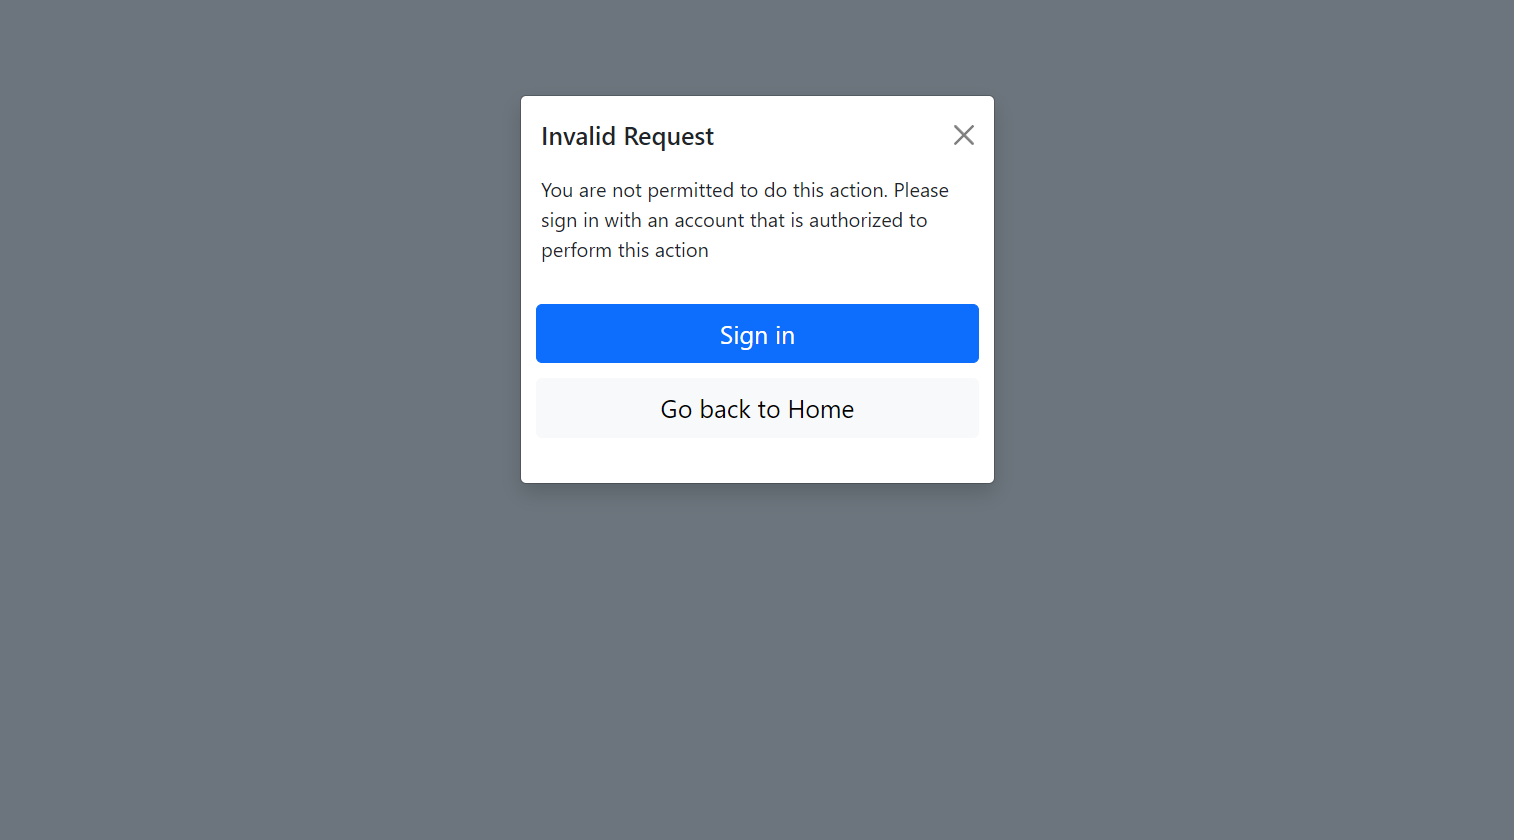
\includegraphics[width=.99\linewidth]{sc1.png}
		\caption{Σελίδα AuthorizationError}
		\label{fig:sub1}
	\end{subfigure}%
	\begin{subfigure}{.5\textwidth}
		\centering
		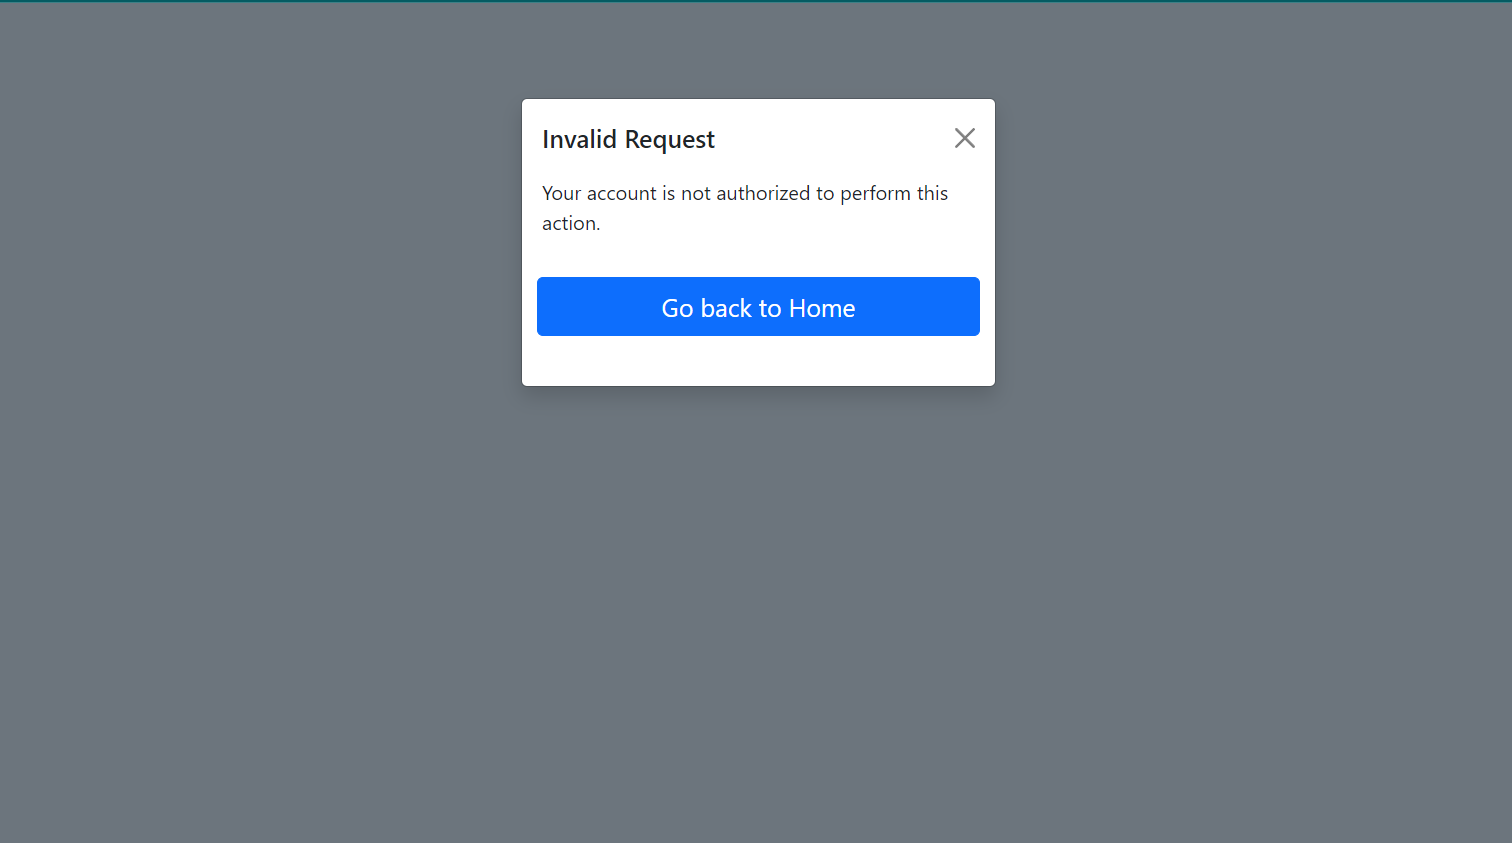
\includegraphics[width=.99\linewidth]{sc2.png}
		\caption{Σελίδα NoRightsError}
		\label{fig:sub2}
	\end{subfigure}
	\caption{}
	\label{fig:test}
\end{figure}



Μια σημαντική λεπτομέρεια που δεν εξηγήθηκε στον κώδικα της προηγούμενης μεθόδου είναι ποιος είναι ο ρόλος του tag:

\begin{minted}
	[
	frame=lines,
	framesep=2mm,
	baselinestretch=1.2,
	bgcolor=LightGray,
	fontsize=\footnotesize
	]{csh}
[ResponseCache(NoStore = true, Location = ResponseCacheLocation.None)]
	\end{minted}
Το συγκεκριμένο tag τοποθετήθηκε στην μέθοδο ώστε το View που επιστρέφεται στον Browser να μην αποθηκεύεται στην cache. Έτσι αν το session λήξει ή ο χρήστης κάνει log out, δεν θα είναι προσβάσιμες οι σελίδες που φορτώθηκαν αν χρησιμοποιηθεί η εντολή "πίσω" του browser.

Τέλος, πρέπει να εξηγηθεί πώς ένας χρήστης μπορεί να αποσυνδεθεί (να κάνει log out) από τον λογαριασμό του όταν ολοκληρώσει τις ενέργειές του. Η λήξη της συνόδου από τον χρήστη γίνεται από την συνάρτηση Logout του HomeController.

\begin{minted}
	[
	frame=lines,
	framesep=2mm,
	baselinestretch=1.2,
	bgcolor=LightGray,
	fontsize=\footnotesize
	]{csh}
public ActionResult Logout()
{
	HttpContext.Session.Clear();
	HttpContext.Session.Remove("username");
	HttpContext.Session.Remove("userid");
	HttpContext.Session.Remove("role");
	return RedirectToAction("Index");
}
\end{minted}

Όπως φαίνεται η συγκεκριμένη μέθοδος αφαιρεί όλα τα πεδία που εισάχθηκαν στο session κατά την είσοδο και ανακατευθύνει τον χρήστη στην αρχική σελίδα Home page.

\subsection{Layout Razor View}
Βασικό μέρος του presentation layer (ή αλλιώς View layer) είναι το \textbf{\_Layout.cshtml}. Το αρχείο αυτό περιλαμβάνεται στον φάκελο Shared και φορτώνεται μαζί με κάθε View Που εμφανίζεται στον browser. Στο αρχείο αυτό γίνεται import το css αρχείο του Bootstrap Framework. Πιο συγκεκριμένα δεν χρησιμοποιήθηκε το css αρχείο που ήδη περιλαμβάνεται στο Visual Studio, αλλά ένα Custom Themed Bootstrap css που δίνει πιο ιδανικά χρώματα σε όλη την εφαρμογή.

Επιπλέον στο \textbf{\_Layout.cshtml} περιλαμβάνεται η μπάρα περιήγησης ή αλλιώς navigation bar. Η συγκεκριμένη μπάρα έχει στα αριστερά 3 συνδέσμους: έναν για το Home page, έναν για το News και έναν για το About page. Οι σελίδες αυτές ανήκουν στον HomeController και θα αναλυθούν σε λίγο. Πιο μεγάλη βαρύτητα έχει ο σύνδεσμος του navbar που βρίσκεται στα δεξιά καθώς όπως φαίνεται στο κώδικα μέσω συνθηκών if αλλάζει ανάλογα με το αν ο χρήστης είναι ή όχι συνδεδεμένος.

%\begin{figure}[H]
%	\centering
%	\begin{subfigure}{.22\textwidth}
%		\centering
%		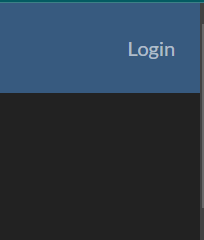
\includegraphics[width=.75\linewidth]{b0.png}
%		\caption{Navbar χωρίς συνδεδεμένο χρήστη}
%		\label{fig:sub21}
%	\end{subfigure}%
%	\begin{subfigure}{.22\textwidth}
%		\centering
%		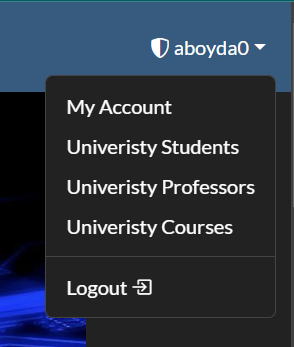
\includegraphics[width=.8\linewidth]{b1.png}
%		\caption{Μενού επιλογών του Γραμματέα}
%		\label{fig:sub22}
%	\end{subfigure}
%		\begin{subfigure}{.22\textwidth}
%		\centering
%		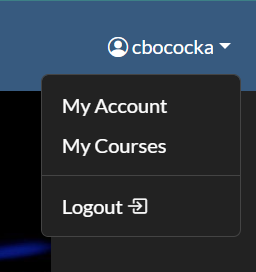
\includegraphics[width=.8\linewidth]{b2.png}
%		\caption{Μενού επιλογών του Καθηγητή}
%		\label{fig:sub23}
%	\end{subfigure}
%	\begin{subfigure}{.22\textwidth}
%		\centering
%		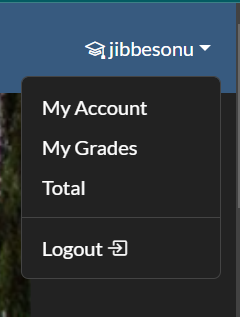
\includegraphics[width=.8\linewidth]{b3.png}
%		\caption{Μενού επιλογών του Φοιτητή}
%		\label{fig:sub24}
%	\end{subfigure}
%	\caption{}
%	\label{fig:test1}
%\end{figure}


\begin{figure}[H]
	\centering
	\begin{subfigure}{.35\textwidth}
		\centering
		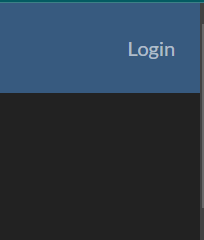
\includegraphics[width=.7\linewidth]{b0.png}
		\caption{Navbar χωρίς συνδεδεμένο χρήστη}
		\label{fig:sub21}
	\end{subfigure}%
	\begin{subfigure}{.35\textwidth}
		\centering
		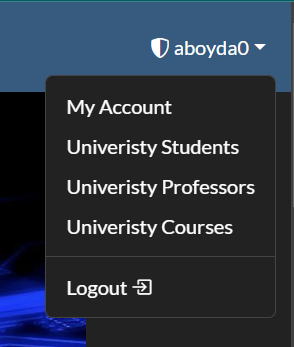
\includegraphics[width=.7\linewidth]{b1.png}
		\caption{Μενού επιλογών του Γραμματέα}
		\label{fig:sub22}
	\end{subfigure}
	\caption{}
	\label{fig:test1}
\end{figure}


\begin{figure}[H]
	\centering
	\begin{subfigure}{.35\textwidth}
		\centering
		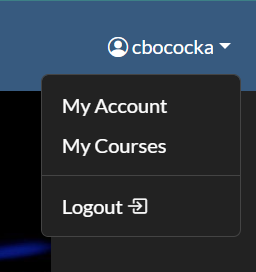
\includegraphics[width=.8\linewidth]{b2.png}
		\caption{Μενού επιλογών του Καθηγητή}
		\label{fig:sub23}
	\end{subfigure}
	\begin{subfigure}{.35\textwidth}
		\centering
		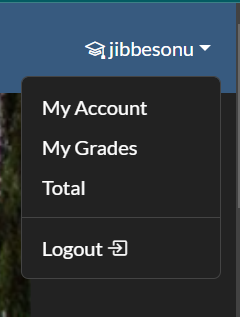
\includegraphics[width=.8\linewidth]{b3.png}
		\caption{Μενού επιλογών του Φοιτητή}
		\label{fig:sub24}
	\end{subfigure}
	\caption{}
	\label{fig:test1}
\end{figure}

Αν ο χρήστης δεν έχει συνδεθεί τότε ο σύνδεσμος απλά τον πάει στο Log in page. Αν όμως ο χρήστης έχει συνδεθεί, τότε ο σύνδεσμος αντικαθίσταται με ένα μενού επιλογών. Το μενού περιέχει όλες τις βασικές σελίδες που αντιστοιχούν στον συγκεκριμένο τύπο χρήστη καθώς και την επιλογή Log out. Ο τίτλος του μενού έχει το username του χρήστη.

Στο κάτω μέρος της σελίδας υπάρχει και ένας footer που περιέχει το όνομα της εφαρμογής και ένα λινκ για την σελίδα License.

\subsection{Home Controller}
Ο HomeController είναι υπεύθυνος για να φορτώνει τις "στατικές" σελίδες της εφαρμογής και αυτές είναι η Index, η News, η About, η Login και η License. Οι σελίδες αυτές αναφέρονται ως στατικές καθώς δεν δέχονται δεδομένα από την βάση δεδομένων της εφαρμογής.

Οι μέθοδοι του HomeController είναι αρκετά απλές με εξαίρεση την POST Login και την GET Logout οι οποίες έχουν ήδη αναλυθεί σε προηγούμενη ενότητα καθώς αφορούν το Session Management. Οι υπόλοιπες μέθοδοι απλά επιστρέφουν το αντίστοιχο View.

Σχετικά με τα Views του HomeController έχουν να επισημανθούν τα εξής:

\begin{itemize}
	
	\item \textbf{Index}:\\
	Αποτελεί την κεντρική σελίδα (Home page) της εφαρμογής. Σε αυτήν εμφανίζονται σύντομες και γενικές πληροφορίες για το Πανεπιστήμιο για το οποίο φτιάχτηκες η εφαρμογή. Στη συγκεκριμένη περίπτωση θεωρείται ότι το πανεπιστήμιο είναι το Πανεπιστήμιο Πειραιά. Η σελίδα αυτή βασίστηκε στο παράδειγμα Carousel της σελίδας Bootstrap.
	
	\item \textbf{News}:\\
	Σε αυτή τη σελίδα περιέχονται τα νέα του πανεπιστημίου. Για λόγους απλότητας το κείμενο είναι hardcoded μέσα στην ίδια σελίδα.
	
	\item \textbf{About}:\\
	Σε αυτή περιέχονται τα ονόματα των δημιουργών της εφαρμογής με συνδέσμους στους λογαριασμούς Github.

	\item \textbf{Login}:\\
	Αποτελεί την σελίδα απ' όπου ο χρήστης θα κάνει Login. Σε αντίθεση με τα άλλα Views γίνεται στο πάνω μέρος του αρχείου η δήλωση:
	
\begin{minted}
	[
	frame=lines,
	framesep=2mm,
	baselinestretch=1.2,
	bgcolor=LightGray,
	fontsize=\footnotesize
	]{csh}
@{
	Layout = null;
}
\end{minted}
	Με αυτό τον τρόπο δεν θα υπάρχει το navbar σε αυτή τη σελίδα (καθαρά για λόγους αισθητικής).

	\item \textbf{License}:\\
	Σε αυτή τη σελίδα περιέχεται η Open Source άδεια της εφαρμογής.

\end{itemize}

Στις ενότητες που ακολουθούν, παρουσιάζονται με λεπτομέρεια οι Controllers που αφορούν τις λειτουργίες των χρηστών.

\subsection{Students Controller}
	
\subsubsection{Περιγραφή των μεθόδων}

\begin{itemize}
	
	\item \textbf{Μέθοδος Index()}\\
	Η μέθοδος αυτή καλείται όταν ο χρήστης συνδεθεί επιτυχώς σαν Φοιτητής. Μόνος ρόλος της είναι να ανακατευθύνει τον χρήστη στην Account Μέθοδο.			
	
	\item	\textbf{Μέθοδος Account()}\\
	Η μέθοδος ανακτά το Student object που αντιστοιχεί στον συνδεδεμένο μαθητή και επιστρέφει το Account View με τον μαθητή ως παράμετρο. Το Account View αποτελεί την σελίδα καλωσόρισης του Φοιτητή. Επιπλέον περνάει στο View (μέσω ViewData) το σύνολο τον E.C.T.s του φοιτητή και τον αριθμό των δηλωμένων μαθημάτων του για να εμφανιστούν στη σελίδα σαν ενημερωτικές πληροφορίες
	
	\item \textbf{Μέθοδος StudentGetter()}\\		
	Η μέθοδος StudentGetter είναι βοηθητική. Στόχος της είναι να αναζητά και επιστρέφει τον μαθητή που είναι συνδεδεμένος αυτή τη στιγμή.\\
	Αρχικά αποθηκεύει το userid που βρίσκεται στο Session και αναζητάει τον μαθητή με το συγκεκριμένο userid. Τέλος, επιστρέφει τον συνδεμένο μαθητή και συμπεριλαμβάνει μαζί τα μοντέλα Courses και CourseHasStudent (μέσω easy loading) για να έχουμε στην πρόσβαση μας τους βαθμούς και τα ονόματα των μαθημάτων του.

	\item \textbf{Μέθοδος Grades(string? sortOrder)}\\
	Η μέθοδος εμφανίζει όλα τα μαθήματα του συνδεδεμένου φοιτητή σε ένα View ταξινομημένα με βάση το εξάμηνο σε αύξουσα σειρά σε ένα Boostrap πίνακα. Δέχεται σαν παράμετρο το sortOrder μέσω του οποίο μπορεί να ταξινομηθεί σε δεύτερο βήμα (OrdeBy ThenBy) μία στήλη του πίνακα στο View. Η ταξινόμηση γίνεται όταν ο χρήστης κάνει κλικ στα κουμπιά που είναι στην επικεφαλίδα της κάθε στήλης του πίνακα Boostrap.
	
 	 \begin{figure}[H]
	\centering
	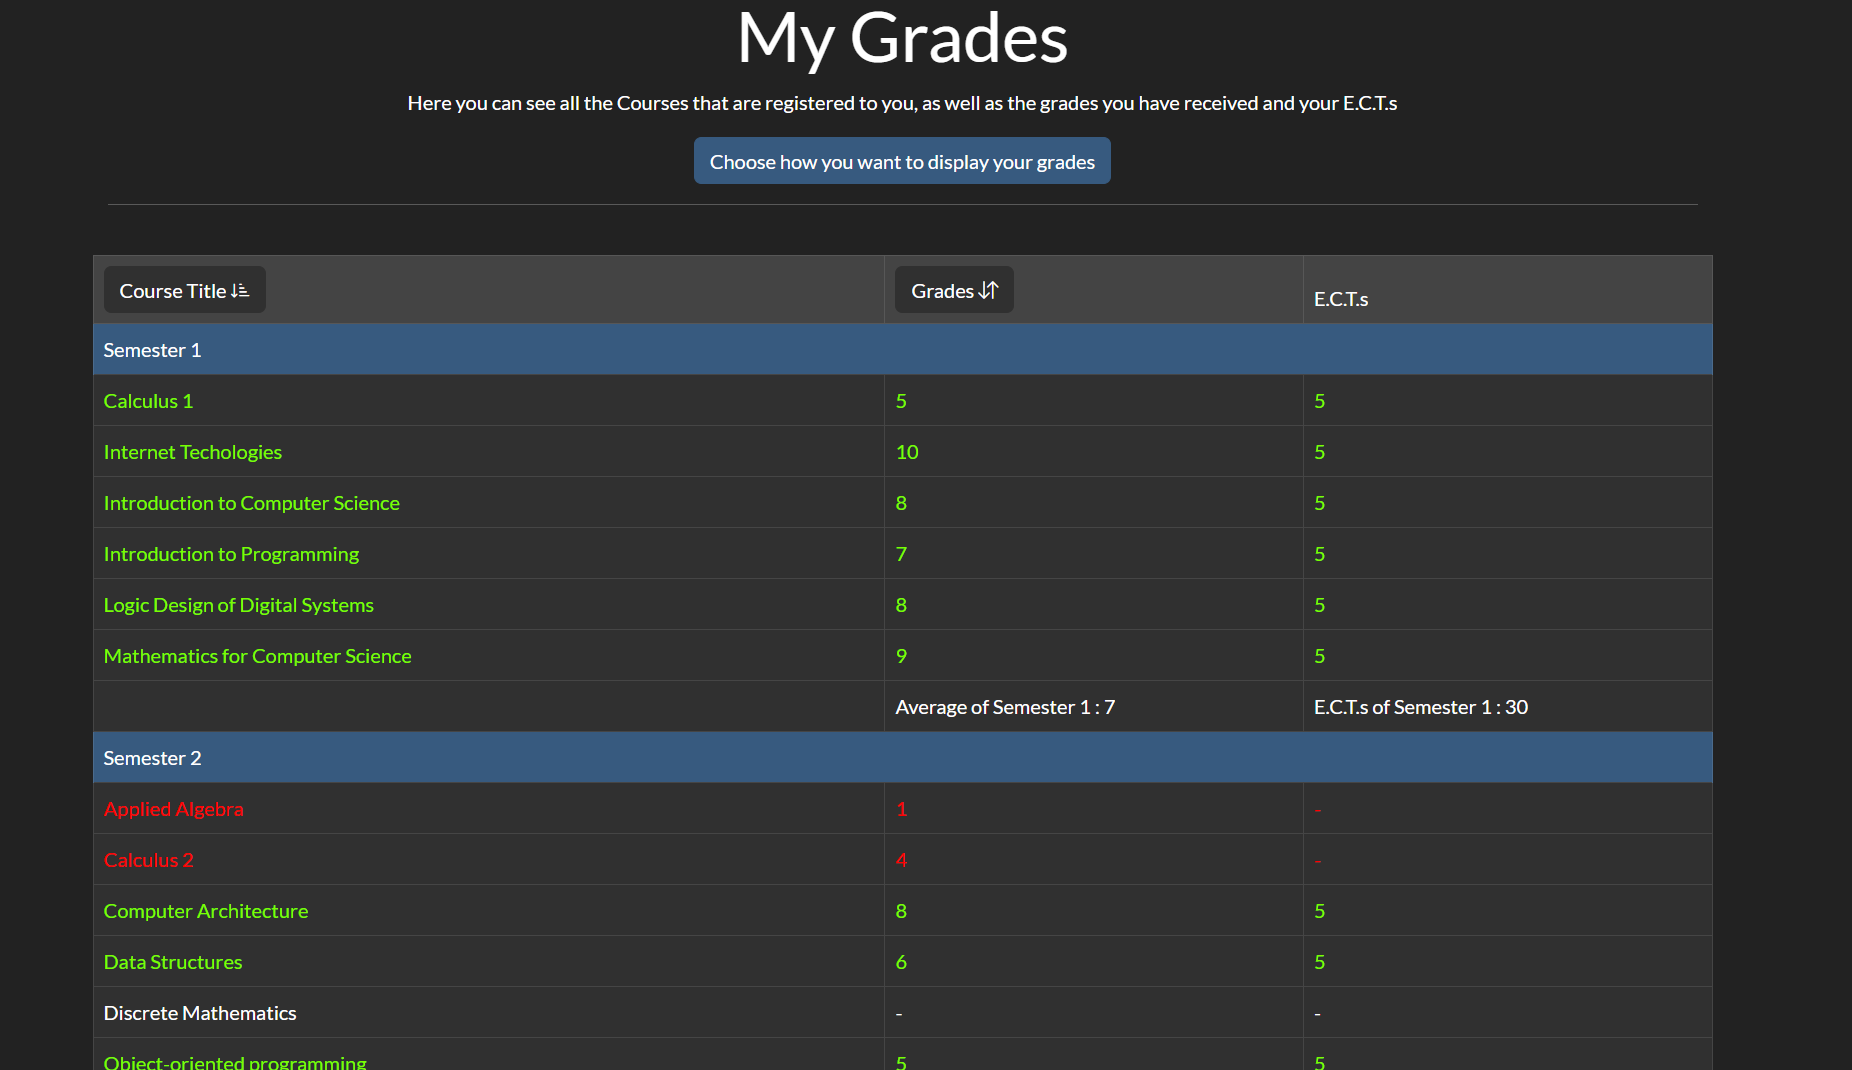
\includegraphics[width=0.75\textwidth]{grades.png}
	\caption{Παράδειγμα του Grades View }
	\label{fig:emptyView}
	\end{figure}

	
	\item \textbf{Μέθοδος Semesters(int? semester)}\\
	Η μέθοδος έχει ως παράμετρο τo εξάμηνο που έχει επιλέξει ο μαθητής για να δει τα μαθήματά του. Αρχικά, ανακτά τον συνδεδεμένο μαθητή και έπειτα αναζητάει τα μαθήματα που είναι στο ίδιο αριθμό εξάμηνου με την μεταβλητή semester. Αν η μεταβλητή semester είναι null τότε την ορίζουμε με τον αριθμό 1 ,δηλαδή τα μαθήματα του πρώτου εξάμηνου. Από σύμβαση θεωρείται ότι υπάρχουν 8 εξάμηνα συνολικά, άρα αν δοθεί semester μεγαλύτερο του 8 θα οριστεί ως 8. Τέλος επιστρέφεται το ανάλογο View με παράμετρο το μοντέλο CourseHasStudents (στη συγκεκριμένη περίπτωση θα είναι λίστα από μοντέλα CourseHasStudents).
		
	\item \textbf{Μέθοδος Total()}\\
	Η μέθοδος αρχικά με την συνάρτηση StudentGetter ανακτά τον συνδεμένο φοιτητή. Έπειτα αποθηκεύει σε μεταβλητές τον αριθμό των δηλωμένων μαθημάτων, των περασμένων μαθημάτων , τον αριθμό των E.C.T.s και την συνολική βαθμολογία (μέσο ορό). Οι μεταβλητές αυτές περνάνε στο αντίστοιχο View (μέσω του ViewData).
	
\end{itemize}

\subsubsection{Σενάριο Εκτέλεσης}
Ο φοιτητής κάνει log in με τα credentials του και ανακατευθύνεται στην σελίδα Account που περιέχει τα στοιχεία του. Έπειτα πατάει πάνω δεξιά στο όνομα του και κάνει κλικ στο  dropdown menu που λέει 'My Grades'. Εκεί προβάλλονται οι βαθμοί του φοιτητή ανά εξάμηνο (μέσω της σελίδας Semesters).  Αν θέλει να δει άλλο εξάμηνο πατάει πάνω στο ανάλογο radio button. Στην συγκεκριμένη σελίδα ο χρήστης μπορεί να πατήσει στο κουμπί \textbf{'Choose how you want to display your grades'} και να πατήσει στο κουμπί \textbf{'View Grades by Title'} για να δει όλα τα μαθήματα ταξινομημένα με βάση το ονόματα των μαθημάτων (μέσω της σελίδας Grades) . Επίσης μπορεί να πατήσει αν θέλει να προβληθούν τα μαθήματα σε αύξουσα ή φθίνουσα σειρά σε κάθε εξάμηνο (ως προς τον τίτλο ή τον βαθμό). 

Στη συνέχεια μπορεί να πατήσει στο dropdown menu την επιλογή Total για να δει την συνολική του βαθμολογία. Τέλος ο φοιτητής μπορεί να κάνει log out από το ίδιο dropdown menu.
	
\subsection{Professors Controller}


\begin{itemize}
	
	\item \textbf{Μέθοδος Index()}\\
	Η μέθοδος αυτή καλείται όταν ο χρήστης συνδεθεί επιτυχώς σαν Καθηγητής. Μόνος ρόλος της είναι να ανακατευθύνει τον χρήστη στην Account Μέθοδο.			
	
	\item \textbf{Μέθοδος Account()}\\
	Η μέθοδος ανακτά το Professor object που αντιστοιχεί στον συνδεδεμένο καθηγητή και επιστρέφει το Account View με τον καθηγητή ως παράμετρο. Το Account View αποτελεί την σελίδα καλωσόρισης του καθηγητή. Επιπλέον περνάει στο View (μέσω ViewData) το τον αριθμό των μαθημάτων που έχουν ανατεθεί στον καθηγητή καθώς και τον αριθμό μαθημάτων που περιέχουν φοιτητές που δεν έχουν λάβει ακόμη τον βαθμό τους. Οι τιμές αυτές θα εμφανιστούν στη σελίδα σαν ενημερωτικές πληροφορίες. Επιπλέον υπολογίζεται και ο αριθμός των μαθημάτων που περιέχουν φοιτητές, καθώς υπάρχει το ενδεχόμενο ένα μάθημα να μην έχει δηλωμένο κανέναν φοιτητή. Έτσι το View θα εμφανίσει κατάλληλο μήνυμα αν πράγματι υπάρχουν μαθήματα με δηλωμένους φοιτητές που δεν έχουν λάβει γραπτό.
	
	\item \textbf{Μέθοδος ProfessorCourses(string? sortOrder)}\\
 	Η μέθοδος αυτή είναι υπεύθυνη για την εμφάνιση όλων των μαθημάτων που έχουν ανατεθεί στον καθηγητή που έχει συνδεθεί. Τα μαθήματα περνάνε στο View ως μία λίστα από Course Models και εμφανίζονται σε ένα bootstrap table. Δεν υλοποιήθηκε pagination καθώς θεωρήθηκε πώς δεν πρόκειται ένας καθηγητής να έχει πάρα πολλά μαθήματα ανατεθειμένα σε αυτόν. Αν ο καθηγητής δεν έχει κανένα μάθημα ανατεθειμένο σε αυτόν τότε δεν εμφανίζεται το bootstrap table αλλά ένα σχετικό μήνυμα.
 	
 	 \begin{figure}[H]
 		\centering
 		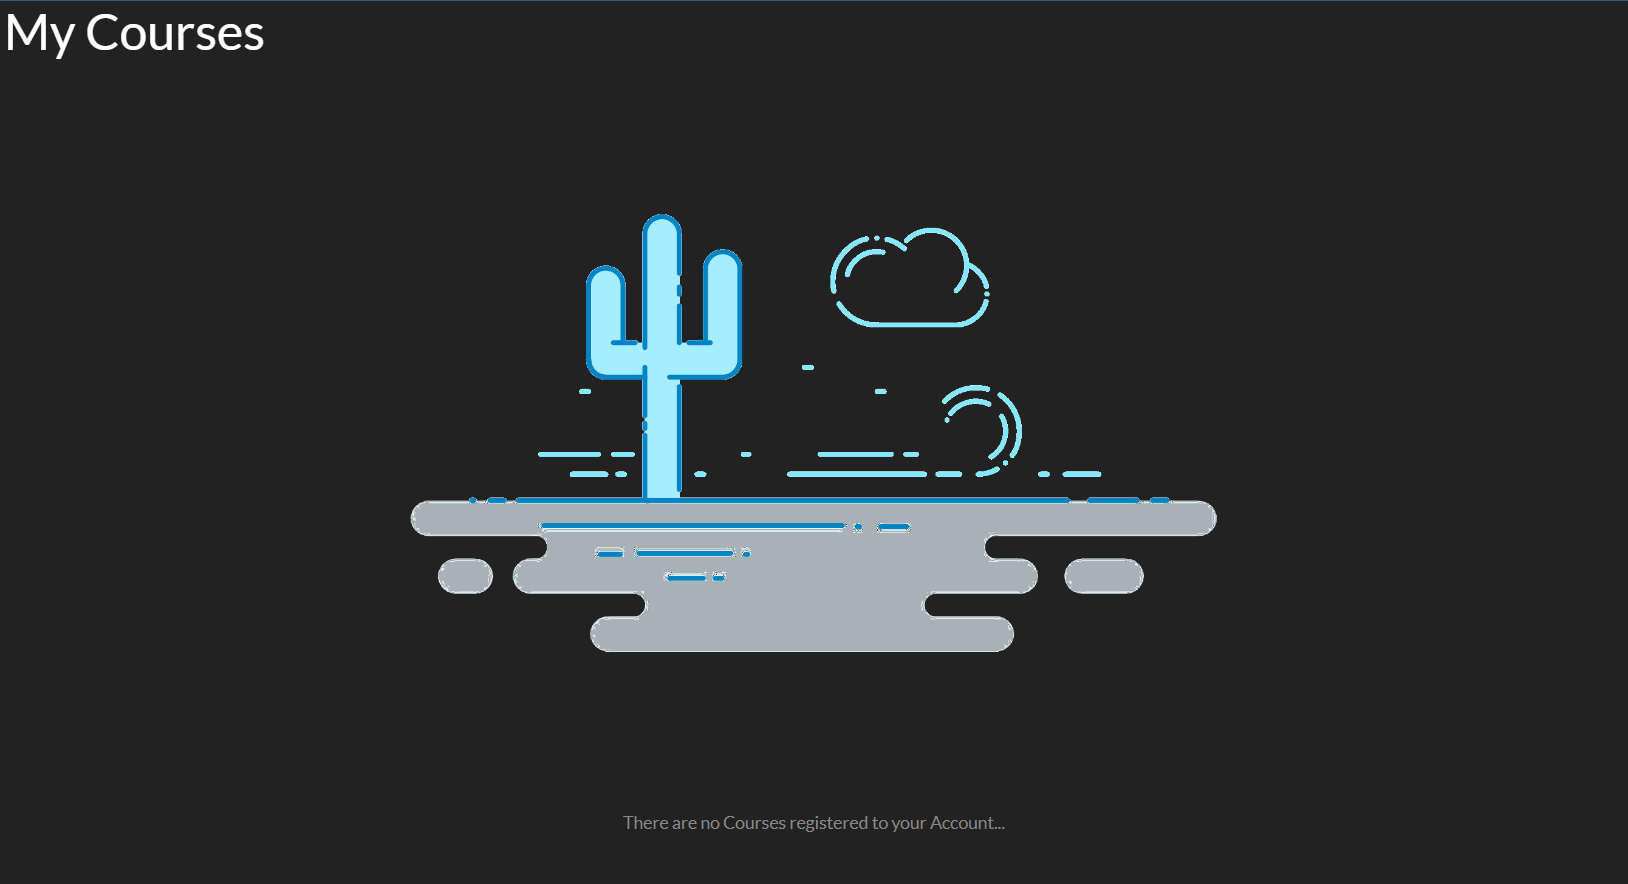
\includegraphics[width=0.72\textwidth]{emptyView.png}
 		\caption{ProfessorCourses View όταν ο καθηγητής δεν έχει κανένα μάθημα ανατεθειμένο σε αυτόν}
 		\label{fig:emptyView}
 	\end{figure}
 	
 	Το bootstrap table αποτελείται από τις στήλες 'Title', 'Semester' και 'Number of Non-Graded Students'. Στον τίτλο της κάθε στήλης υπάρχει και ένα κουμπί το οποίο αν πατήσει ο χρήστης θα ταξινομηθεί ο πίνακας ως προς αυτή την στήλη. Η ταξινόμηση γίνεται Server side. Η μέθοδος δέχεται μία παράμετρο sortOrder η οποία δηλώνει τη στήλη και την σειρά ταξινόμησης. Αν δεν δοθεί τιμή στη παράμετρο τότε γίνεται ταξινόμηση (σε αύξουσα σειρά) στη στήλη 'Title'.
 	
 	Κάθε κουμπί στη πρώτη γραμμή του bootstrap table περιέχει και ένα εικονίδιο το οποίο δηλώνει αν η συγκεκριμένη είναι ή όχι ταξινομημένη και αν ναι, ως προς ποια στήλη είναι ταξινομημένη. Η μέθοδος φροντίζει να συντηρεί κατάλληλες τιμές στο Dictionary του View (δηλαδή στα ViewData) ώστε να λειτουργούν σωστά τα κουμπιά.
 	
 	\begin{figure}[H]
 		\centering
 		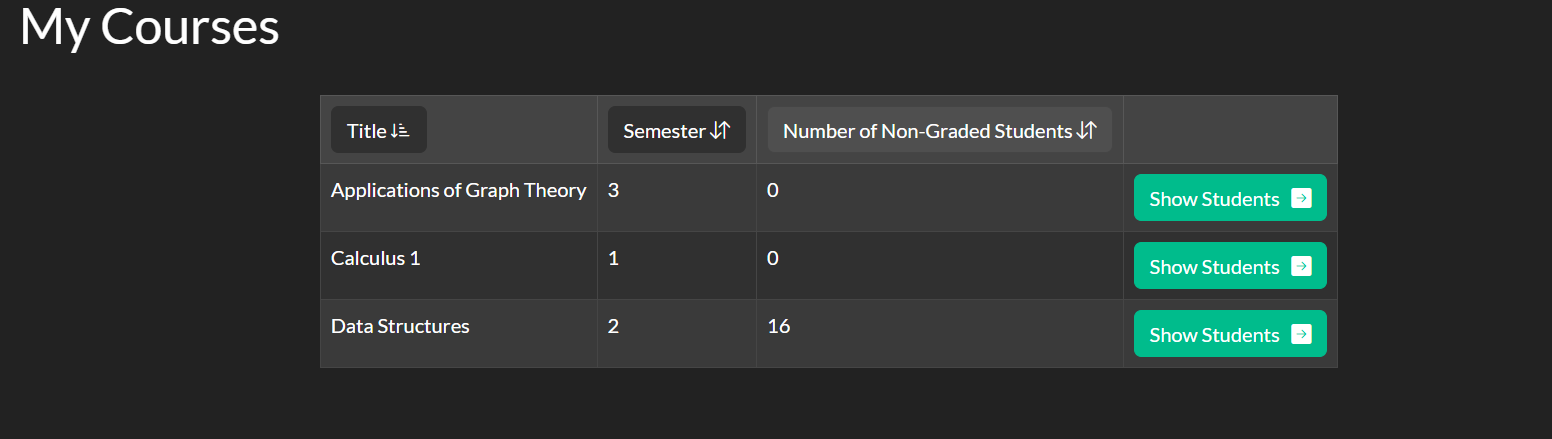
\includegraphics[width=0.72\textwidth]{table1.png}
 		\caption{Παράδειγμα του πίνακα bootstrap στο View ProfessorCourses}
 		%\label{fig:emptyView}
 	\end{figure}
 	
 	Τέλος σε κάθε γραμμή του table που περιέχεται μάθημα, υπάρχει ένα κουμπί το οποίο θα καλέσει την μέθοδο RegisteredStudents για ο συγκεκριμένο μάθημα.
	
	\item \textbf{Μέθοδος RegisteredStudents(int? id, ...)}\\
	Η μέθοδος έχει ως παράμετρο το id του course που έχει επιλέξει ο καθηγητής να δει. Αρχικά ανακτά τον συνδεμένο καθηγητή και αναζητάει το μάθημα που επέλεξε. Αν δεν βρει το μάθημα σημαίνει ότι ο καθηγητής επέλεξε να δει μάθημα που δεν διδάσκει και του εμφανίζεται μήνυμα ότι δεν έχει δικαίωμα να δει το μάθημα (NoRightsError View). Αν ο έλεγχος πετύχει, η μέθοδος βρίσκει τους μαθητές που έχουν δηλώσει το συγκεκριμένο μάθημα του καθηγητή και τους περνάει μέσω μίας λίστας από CourseHasStudents objects. Η λίστα αυτή εμφανίζεται ως ένα bootstrap table στο View.  Παρόμοια με πριν θα εμφανιστεί κατάλληλο μήνυμα αν στο συγκεκριμένο μάθημα δεν υπάρχει κανένας δηλωμένος μαθητής (βλέπε εικόνα \ref{fig:emptyView}).
	
	 \begin{figure}[H]
		\centering
		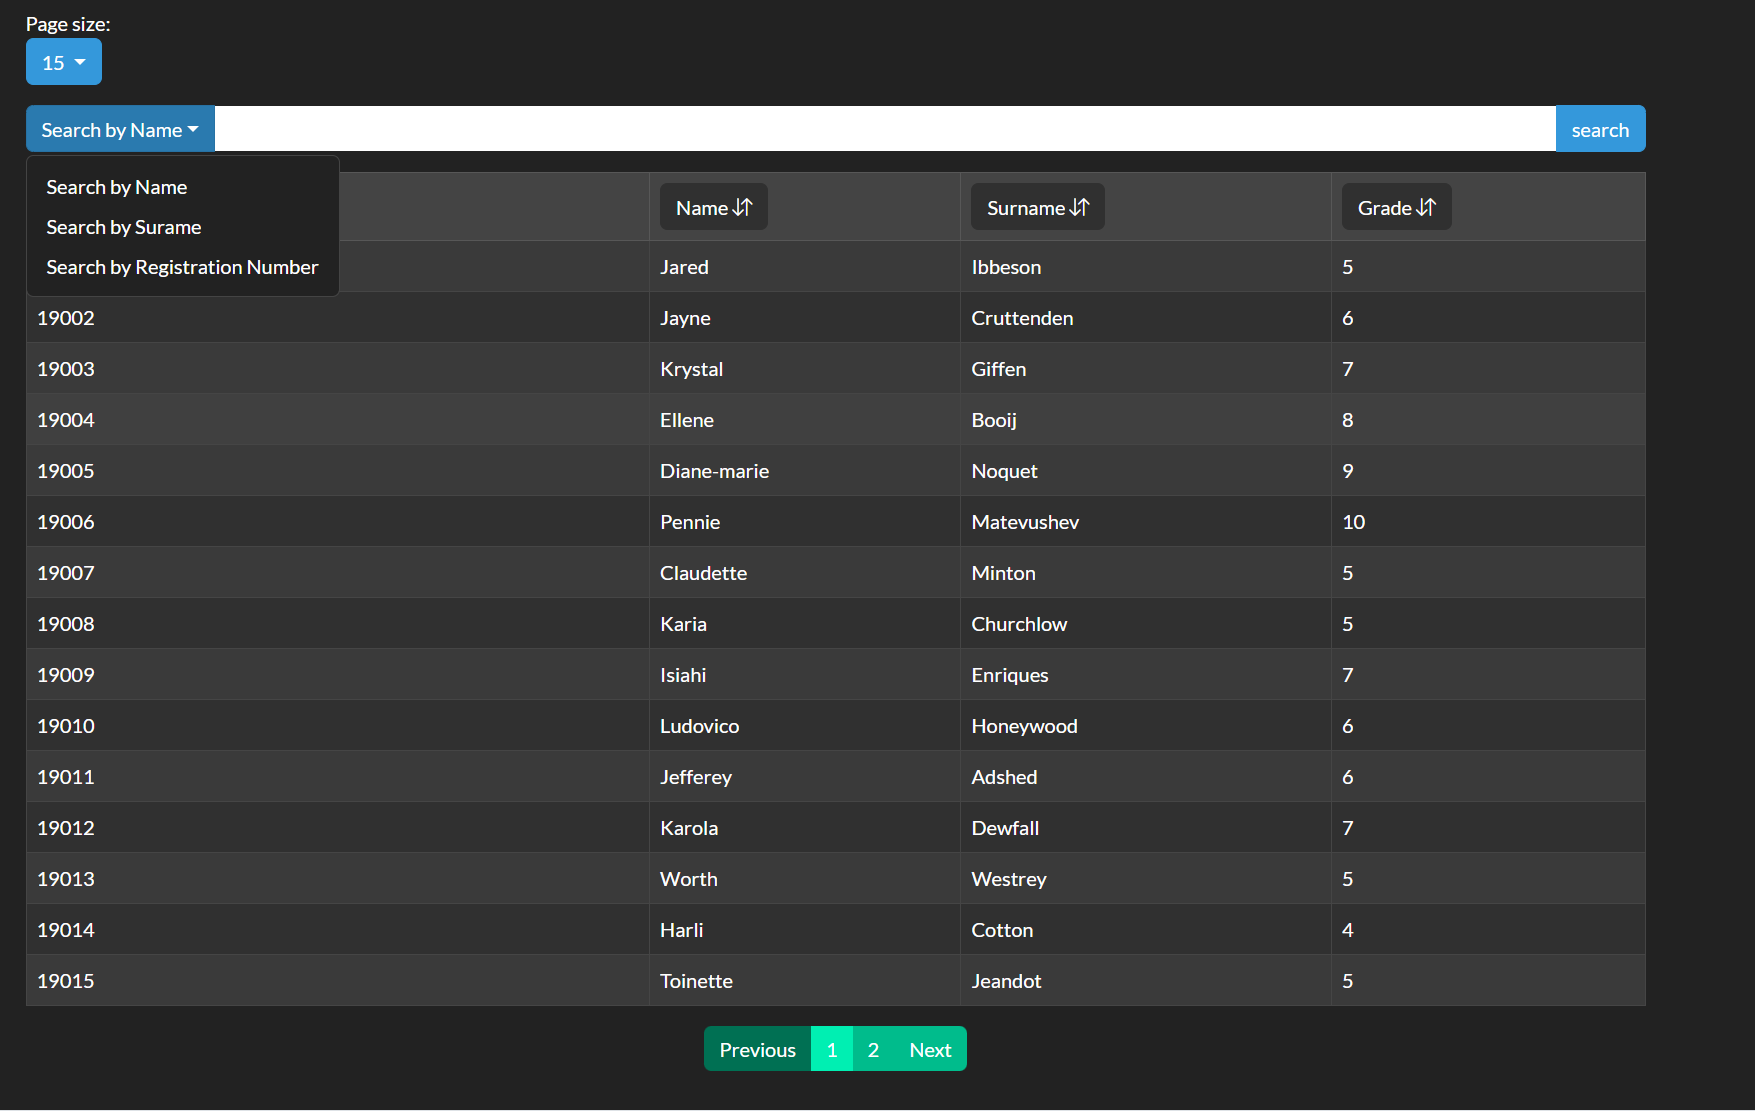
\includegraphics[width=0.85\textwidth]{pages1.png}
		\caption{Παράδειγμα του πίνακα bootstrap στο View RegisteredStudents}
		%\label{fig:emptyView}
	\end{figure}
	
	Το View της συγκεκριμένης μεθόδου έχει αρκετό κώδικα καθώς υποστηρίζει:
	\begin{itemize}
		\item[$\blacksquare$] αναζήτηση με βάση πεδίου
		\item[$\blacksquare$] ταξινόμηση με βάση τη στήλη που επιλέγει ο χρήστης στο bootstrap table
		\item[$\blacksquare$] σελιδοποίηση για την οποία μπορεί ο χρήστης να αλλάξει και το μέγεθος της σελίδας
	\end{itemize}
	
	Η λειτουργικότητα αποτελεί μία επέκταση του παραδείγματος σελιδοποίησης που παρουσιάστηκε στις διαλέξεις του μαθήματος. Όλη η διαδικασία γίνεται server side, όπου η συνάρτηση συντηρεί το Dictionary της σελίδας ώστε να έχει κατάλληλες τιμές για την ταξινόμηση, την αναζήτηση και το μέγεθος της σελίδας. Στο View συμπεριλαμβάνεται και Javascript. Στόχος της είναι να αλλάζει το text στο dropdown πεδίο από το οποίο ο χρήστης επιλέγει ως προς ποια παράμετρο θα κάνει αναζήτηση. 
	
	 \begin{figure}[H]
		\centering
		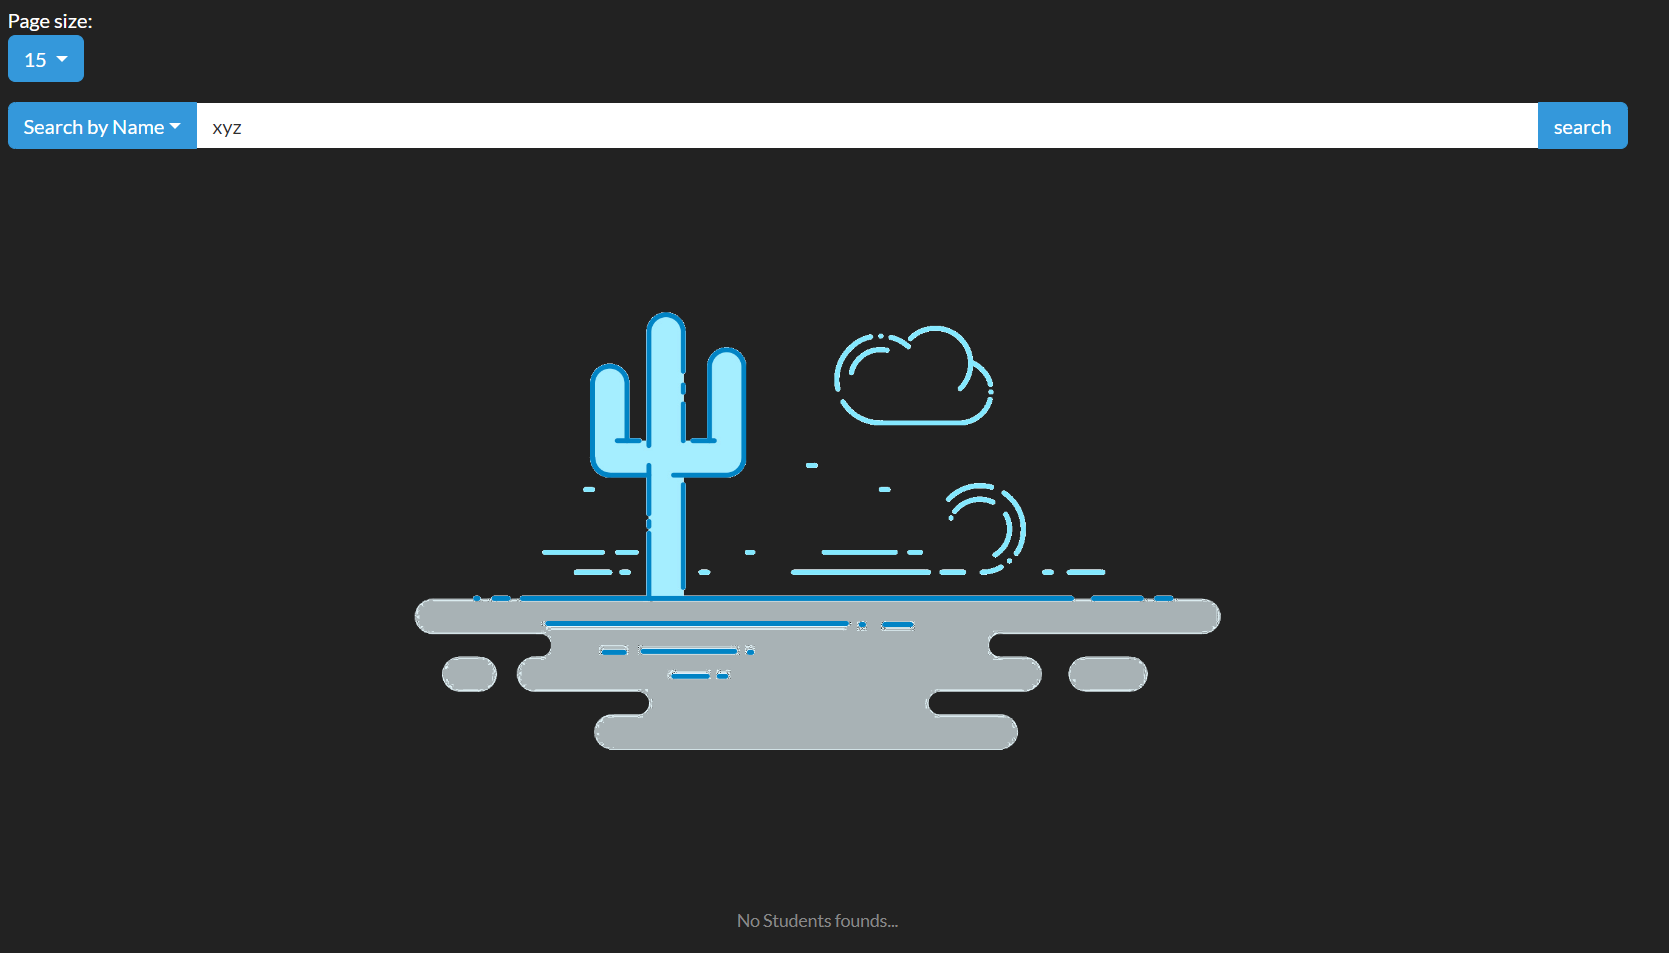
\includegraphics[width=0.7\textwidth]{empty2view.png}
		\caption{Παράδειγμα στο View RegisteredStudents όπου η αναζήτηση του χρήστη δεν είχε κανένα αποτέλεσμα}
		%\label{fig:emptyView}
	\end{figure}
	Τέλος ένα σημαντικό μέρος του View είναι οι επιλογές με τις οποίες ο Καθηγητής μπορεί να ανεβάσει βαθμούς στη βάση.
	
	\begin{figure}[H]
		\centering
		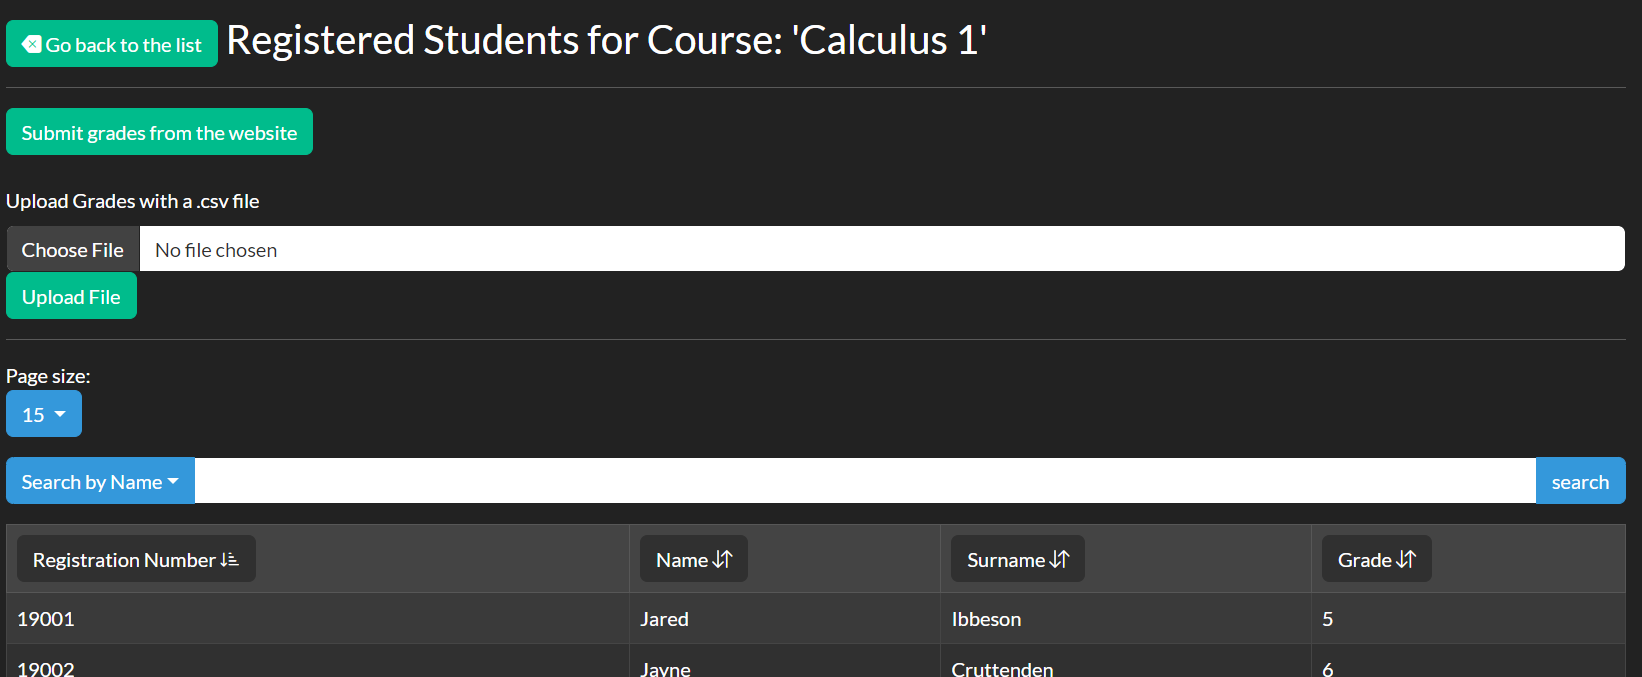
\includegraphics[width=0.85\textwidth]{options.png}
		\caption{Επιλογές στο View RegisteredStudents για ανάρτηση βαθμών}
		%\label{fig:emptyView}
	\end{figure}

	Ο Καθηγητής μπορεί να αναρτήσει βαθμούς για το συγκεκριμένο μάθημα είτε \textbf{μέσω της ιστοσελίδας} (επιλογή 'Submit grades from the website') είτε \textbf{αναρτώντας ένα .csv αρχείο} (επιλογή 'Choose File' και 'Upload File').

	\item \textbf{Μέθοδος UploadGrades(int CourseId, IFormFile usercsv)}\\
	Όταν ο χρήστης αναρτήσει ένα .csv αρχείο από το RegisteredStudents View καλείται η POST μέθοδος UploadGrades. Η μέθοδος έχει ως παραμέτρους το ID του μαθήματος και το .csv αρχείο που περιέχει τους βαθμούς του μαθήματος. Το αρχείο μπορεί να φτιαχτεί μέσω Excel και σε κάθε γραμμή πρέπει να έχει τη δομή:\\ \textbf{<REGISTRATION NUMBER>,<GRADE>} \\

	\begin{figure}[H]
	\centering
	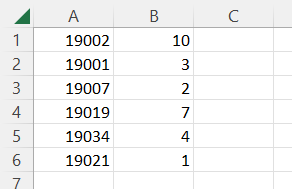
\includegraphics[width=0.25\textwidth]{excel.png}
	\caption{Παράδειγμα ενός έγκυρου .csv αρχείου στο Excel}
	%\label{fig:emptyView}
	\end{figure}
		
	Αρχικά η μέθοδος αντιγράφει το αρχείο στον τοπικό φάκελο Files και στη συνέχεια το ανοίγει και το διαβάζει ανα γραμμή. Η μέθοδος εξετάζει για κάθε μαθητή αν υπάρχει στη βάση δεδομένων, και αν υπάρχει επιβεβαιώνει πως πράγματο έχει δηλώσει το μάθημα. Οι μαθητές που δεν υπάρχουν ή δεν έχουν δηλώσει το μάθημα τους αποθηκεύει σε λίστες για να εκτυπωθούν αργότερα στο View ResultReport. Επιπλέον αν κάποιος φοιτητής έχει μη έγκυρο βαθμό (μικρότερος του 0 ή μεγαλύτερος του 10) αποθηκεύεται επίσης σε λίστα. Αν όμως η εγγραφή του αρχείου είναι σωστή τότε αποθηκεύεται ο βαθμός του στην βάση δεδομένων. 
	
	Τέλος αν δεν υπάρξει λάθος φοιτητής τότε η μέθοδος ανακατευθύνει τον χρήστη στο View του RegisteredStudents, ενώ αν υπάρχουν λάθος φοιτητές στο αρχείο τότε τον ανακατευθύνει στο View ResultReport.
	
	\begin{figure}[H]
		\centering
		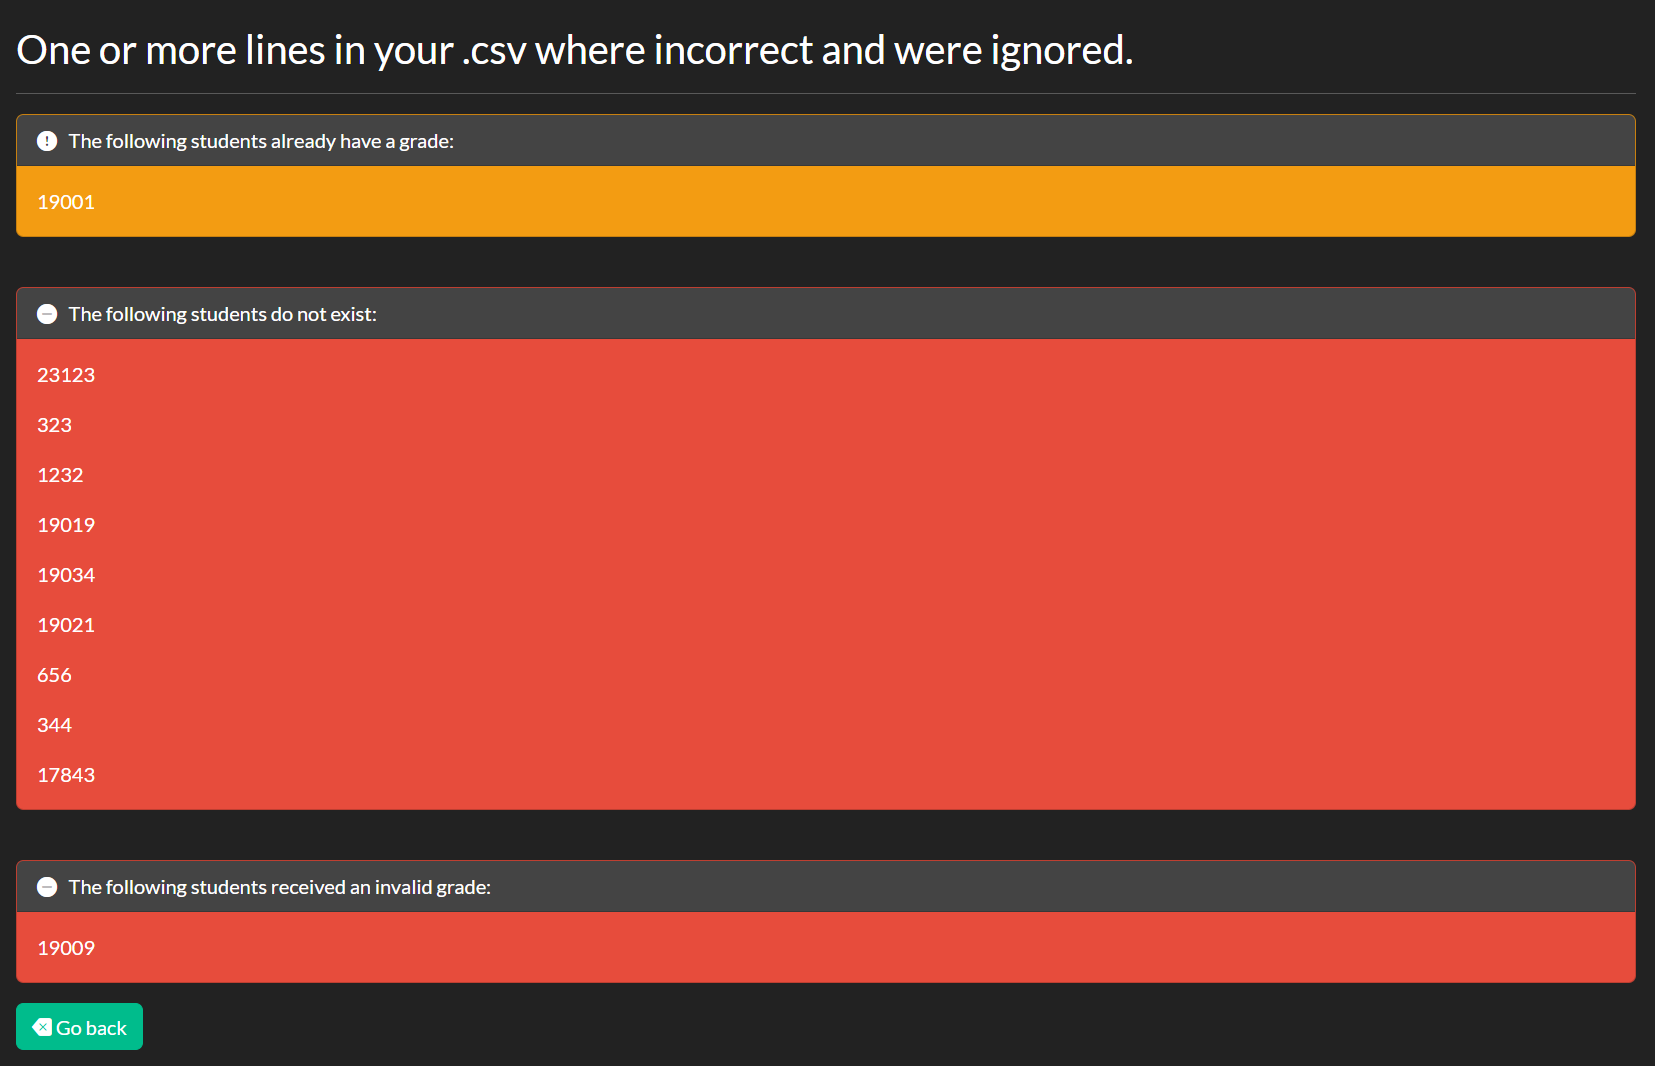
\includegraphics[width=0.75\textwidth]{result.png}
		\caption{Παράδειγμα του View ResultReport}
		%\label{fig:emptyView}
	\end{figure}

	\item \textbf{Μέθοδος EditGrades(int id)}\\
	Όταν ο χρήστης επιλέξει 'Submit grades from the website' από το RegisteredStudents View καλείται η GET μέθοδος EditGrades.
	Η μέθοδος έχει ως παράμετρο το id του μαθήματος που έχει επιλέξει ο καθηγητής. Η μέθοδος ανακτά τους φοιτητές που έχουν δηλωμένο το συγκεκριμένο μάθημα αλλά δεν έχουν βαθμό. Οι φοιτητές ταξινομούνται με βάση το Registration Number και περνάνε στο View.
	
	Το συγκεκριμένο View δεν έχει υλοποιημένο pagination, καθώς δεν υπάρχει συστηματικός τρόπος οι βαθμοί που συμπληρώνει ο καθηγητής σε μία σελίδα να μην χάνονται κάθε φορά που αλλάζει σελίδα. Για απλότητα έχουμε ένα bootstrap table με στήλες '
	Registration Number' και 'Grade'. Στη στήλη 'Grade' υπάρχουν input number που δέχονται τον βαθμό. Μέσω javascript ελέγχεται αν ο καθηγητής δώσει μη έγκυρο βαθμό για έναν φοιτητή (μικρότερος του 0 ή μεγαλύτερος του 10).
	
	\begin{figure}[H]
	\centering
	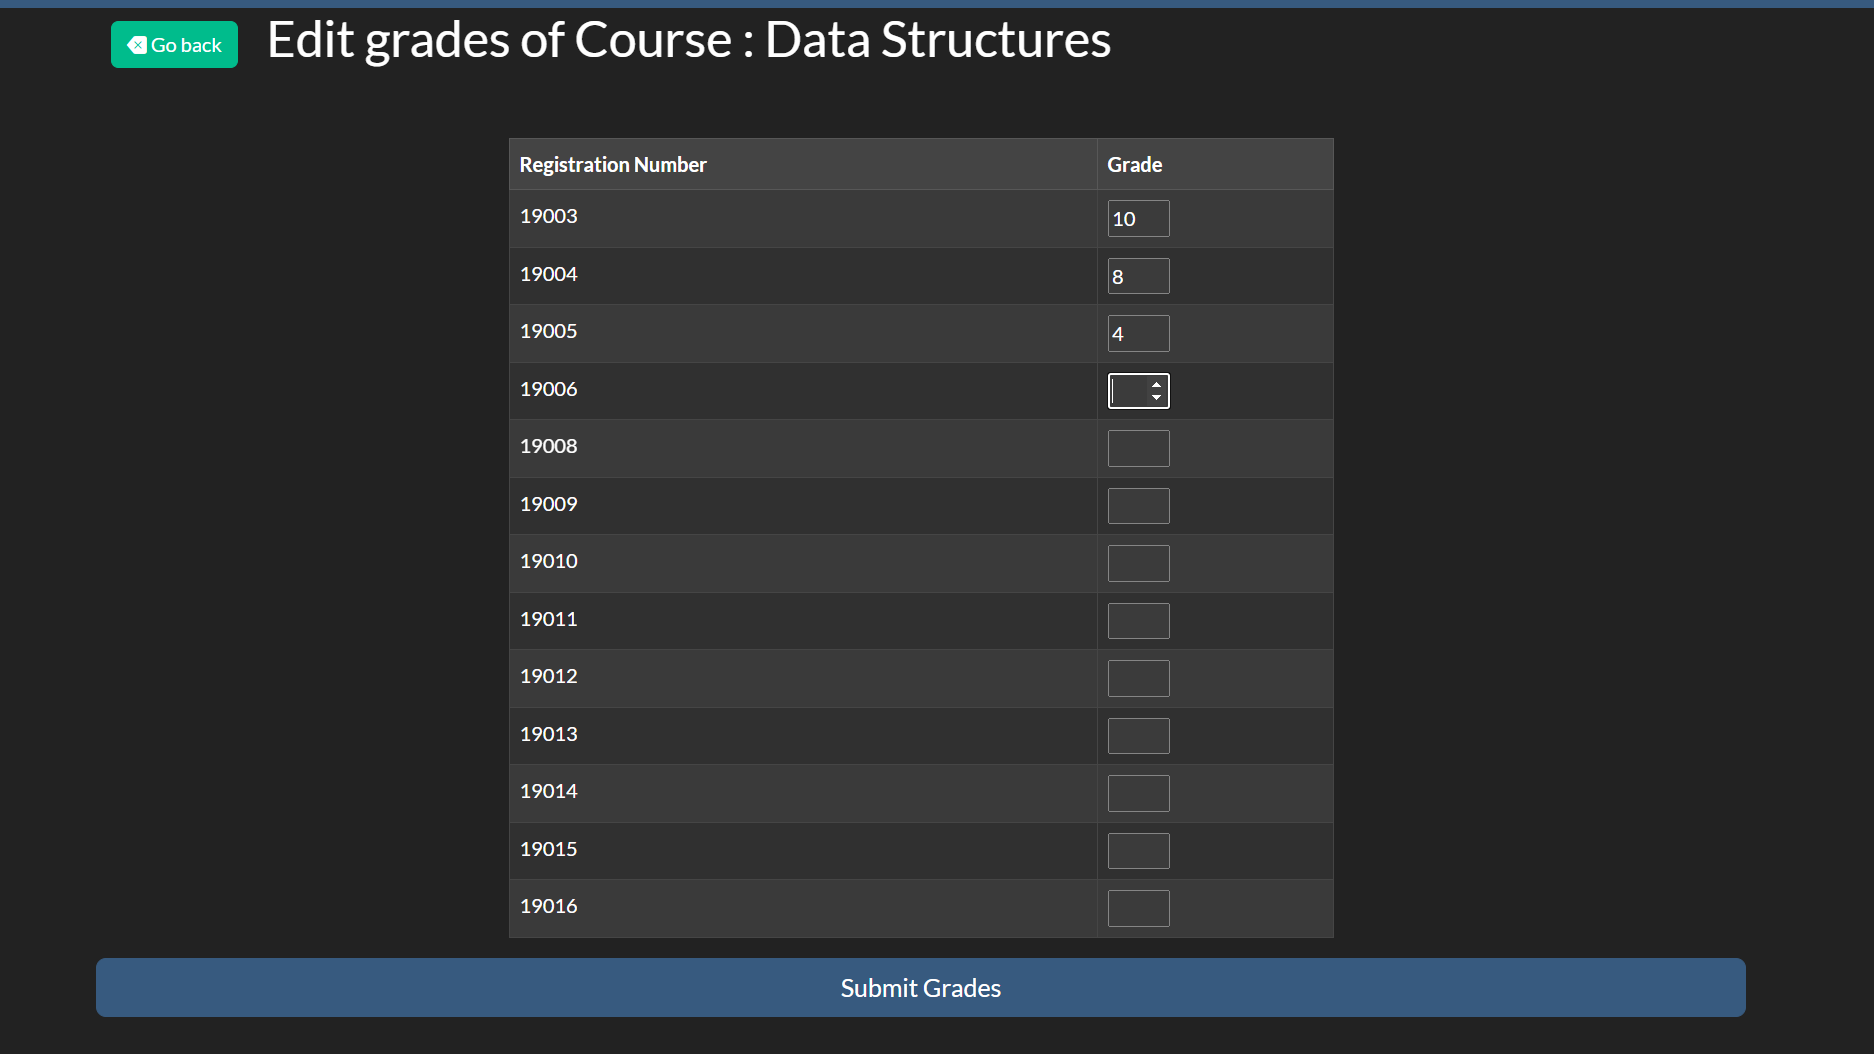
\includegraphics[width=0.75\textwidth]{edits.png}
	\caption{Παράδειγμα του bootstrap table στο View EditGrades}
	%\label{fig:emptyView}
	\end{figure}

	Όταν ο καθηγητής πατήσει 'Submit grades' μέσω javascript όλοι οι βαθμοί συγκεντρόνονται σε ένα string και περνάει ως παράμετρος στη POST EditGrades.
	
	\item \textbf{Μέθοδος EditGrades(int id, string addedGrades)}\\
	Η μέθοδος έχει ως παραμέτρους το id  του μαθήματος που έχει επιλέξει ο καθηγητής και τους βαθμούς των μαθητών που έχει βάλει. Αν η μεταβλητή με τους βαθμούς είναι κενή σημαίνει ότι ο καθηγητής δεν άλλαξε τους βαθμούς και ανακατευθύνει τον καθηγητή στην σελίδα EditGrades. Έπειτα επεξεργάζεται το string με τους βαθμούς και αποθηκεύει τους νέους βαθμούς στην βάση δεδομένων. Τέλος επιστρέφει το View του EditGrades με το id του επιλεγμένου μαθήματος.		
				
\end{itemize}

\subsubsection{Σενάριο Εκτέλεσης}
Ο καθηγητής κάνει log in με τα credentials του και ανακατευθύνεται στην σελίδα Account. Έπειτα πατάει από το dropdown menu την επιλογή My courses και ανακατευθύνεται στα μαθήματα που διδάσκει. Σε κάθε μάθημα υπάρχει ένα κουμπί 'Show Students' με το οποίο όταν το πατήσει δείχνει όλους τους μαθητές που έχουν δηλώσει το μάθημα και εκεί μπορεί να καταχωρίσει τους βαθμούς των μαθητών (είτε μεταβαίνοντας στην EditGrades είτε αναρτώντας ένα.csv με την αντίστοιχη μέθοδο POST). Τέλος ο καθηγητής μπορεί να κάνει log out.

\subsection{Secretaries Controller}

\subsubsection{Περιγραφή των μεθόδων}

\begin{itemize}
	
	\item \textbf{Μέθοδος Index()}\\
	Η μέθοδος αυτή καλείται όταν ο χρήστης συνδεθεί επιτυχώς σαν Γραμματέας. Μόνος ρόλος της είναι να ανακατευθύνει τον χρήστη στην Account Μέθοδο.		
	
	\item \textbf{Μέθοδος Account()}\\
	Η μέθοδος ανακτά το Secretary object που αντιστοιχεί στον συνδεδεμένο γραμματέα και επιστρέφει το Account View με τον γραμματέα ως παράμετρο. Το Account View αποτελεί την σελίδα καλωσόρισης του γραμματέα. Επιπλέον περνάει στο View (μέσω ViewData) το τον αριθμό των μαθημάτων, των φοιτητών και των καθηγητών που είναι στη βάση για να εμφανιστούν σαν πληροφορίες στο View.
	
	\item \textbf{Μέθοδος UniversityCourses()}\\
	Η μέθοδος αυτή είναι υπεύθυνη για την εμφάνιση όλων των μαθημάτων της βάσης δεδομένων σε έναν boostrap πίνακα. Ο πίνακας ταξινομείται ως προς τις στήλες του και γι' αυτό πρέπει η μέθοδος να συντιρεί κατάλληλα το Dictionary του view. Ο χρήστης θα μπορεί να επιλέγει την στήλη ταξινόμησης από το κουμπί στην επικεφαλίδα της κάθε στήλης. Επιπλέον ο πίνακας έχει pagination και αναζήτηση με βάση τον τίτλο του μαθήματος.
	
	Το μόνο σημαντικό σημείο είναι ότι στον πίνακα του View η στήλη Status δηλώνει αν το πεδίο Professor ενός Course είναι ή όχι null (δηλαδή αν το μάθημα έχει δηλωμένο καθηγητή).
	
	\item \textbf{Μέθοδος CreateCourse()}\\
	Η συγκεκριμένη συνάρτηση χρησιμοποιείται για να προβάλει στον χρήστη μια φόρμα δημιουργίας μαθήματος. Στη φόρμα αυτή εμφανίζεται και ένα dropdown menu από το οποίο μπορεί ο χρήστης να επιλέξει τον καθηγητή που θα είναι υπεύθυνος για το μάθημα. Μπορεί επίσης να επιλέξει \textbf{None} και να ορίσει τον καθηγητή εκ των υστέρων. 

	\item \textbf{Μέθοδος CreateCourse(Course course)}\\
	Η μέθοδος χρησιμοποιείται για εισαχθεί το νέο μάθημα στη βάση δεδομένων. Αν δεν έχουν εισαχθεί ακόμα μαθήματα το coursId παίρνει την τιμή 1, ενώ αντίθετα παίρνει την τιμή courseId του τελευταίου μαθήματος στην λίστα συν ένα. Αυτή η διαδικασία ουσιαστικά προσομοιώνει το AUTO INCREMENT μίας βάσης δεδομένων.
	
	Αν τα δεδομένα που έχει γράψει ο γραμματέας είναι έγκυρα τότε δεν εισάγονται στην βάση δεδομένων και η μέθοδος ανακατευθύνει τον χρήστη στο View του UniversityCourses.
	
	\item \textbf{Μέθοδος AssignProfessor(int id)}\\
	Η μέθοδος χρησιμοποιείται για να προβάλει στον χρήστη μια φόρμα με την οποία μπορεί να αναθέσει καθηγητή σε μάθημα που δεν έχει δηλωμένο καθηγητή. Καλείται όταν ο χρήστης πατήσει πάνω ένα μάθημα της λίστας του View 	UniversityCourses το οποίο δεν έχει καθηγητή.		

	\item \textbf{Μέθοδος AssignProfessor(int id, Course course)}\\
	Αυτή η μέθοδος καλείται από την φόρμα του View AssignProfessor.	Αν το Id που δόθηκε δεν είναι το ίδιο με το id μαθήματος που δεν έχει υπεύθυνο καθηγητή  εμφανίζει στον χρήστη μια σελίδα σφάλματος. Αντίθετα, αν το μάθημα υπάρχει στη βάση ενημερώνεται σύμφωνα με την φόρμα.

	\item \textbf{Μέθοδος UniversityStudents(...)}\\
	Η μέθοδος χρησιμοποιείται για να προβάλει στον χρήστη όλους τους φοιτητές του τμήματος. Η μέθοδος και το αντίστοιχο View είναι παρόμοια με το action Method \textbf{RegisteredStudents}. Ο κώδικας περιλαμβάνει pagination, αναζήτηση ως προς ένα πεδίο που καθορίζει ο χρήστης, ταξινόμηση με βάση επιλεγμένη στήλη ακόμη και αλλαγή του μεγέθους της σελίδας του pagination. Ο κώδικας της μεθόδου αποτελεί μία γενική επέκταση του κώδικα που παρουσιάστηκε στις διαλέξεις του μαθήματος.
	
	\item \textbf{Μέθοδος CreateStudent()}\\
	Η μέθοδος χρησιμοποιείται για να προβάλει στο χρήστη φόρμα δημιουργίας μαθητή. Καλείται από το View UniversityStudents.
						
	\item \textbf{Μέθοδος CreateStudent(Student student)}\\
	Η μέθοδος καλείται από το View CreateStudent και χρησιμοποιείται για την εισαγωγή ενός νέου φοιτητή στη βάση δεδομένων. Αν δεν έχουν εισαχθεί ακόμα φοιτητές το  student ID παίρνει την τιμή 1, ενώ αντίθετα παίρνει την τιμή Student ID του τελευταίου φοιτητή στην λίστα συν ένα (το ίδιο ισχύει για το userId του φοιτητή). Παρόμοια με πριν υλοποιείται το AUTO INCREMENT. Αν τα δεδομένα που έχει γράψει ο γραμματέας είναι έγκυρα τότε δημιουργείται ένα νέο model User object και ένα model Student object τα οποία αποθηκεύονται στην βάση δεδομένων.
	
	\item \textbf{Μέθοδος StudentDetails(int? id, int? semester, string? sortOrder)}\\
	Η μέθοδος χρησιμοποιείται για να προβάλει τις πληροφορίες του φοιτητή που επέλεξε ο χρήστης από την λίστα φοιτητών στο View UniversityStudents. Η μέθοδος αρχικά αναζητάει και αποθηκεύει με βάση το id που δόθηκε στη παράμετρο τον φοιτητή. Αν το μοντέλο είναι null σημαίνει ότι δεν βρήκε φοιτητή με το συγκεκριμένο id και εμφανίζει στον χρήστη ανάλογο μήνυμα. Έπειτα αποθηκεύει στο ViewData τα δηλωμένα μαθήματα και τα E.C.T.s του φοιτητή για να τα προβάλει. Τέλος επιστρέφει το View με παράμετρο το μοντέλο Student.
	
	Στο αντίστοιχο View αυτής της μεθόδου υπάρχει ένας πίνακας που δείχνει τα δηλωμένα μαθήματα του φοιτητή. Αξίζει να αναφερθεί πως σε αυτόν τον πίνακα υποστηρίζεται ταξινόμηση με βάση τις στήλες αλλά αντίθετα με τα προηγούμενα action methods, η διαχείρηση της ταξινόμησης γίνεται στο View και όχι στη μέθοδο.
		
	\item \textbf{Μέθοδος StudentAssignCourses(int? id)}\\
	Όταν ο χρήστης είναι στη σελίδα με τις λεπτομέρειες του φοιτητή μπορεί μέσω κουμπιού να καλέσει την μέθοδο StudentAssignCourses ώστε να του αναθέσει μαθήματα.\\
	Η μέθοδος αναζητάει τον φοιτητή που έχει το ίδιο id με την παράμετρο. Αν δεν βρεθεί φοιτητής με το ίδιο id θα εμφανιστεί ανάλογο μήνυμα. Έπειτα αναζητάει τα μαθήματα του φοιτητή και ανακτά τα μαθήματα που δεν έχουν δηλωθεί για τον συγκεκριμένο καθηγητή και τα περνάει στο Dictionary του View.
	
	Το View που εμφανίζεται στον browser έχει σε έναν πίνακα όλα τα μαθήματα που δεν έχει δηλώσει ο φοιτητής. Σε κάθε μάθημα υπάρχει ένα checkbox. O γραμματέας "τσεκάρει" τα μαθήματα που θέλει να δηλώσει για τον συγκεκριμένο καθηγητή και πατάει το κουμπί 'Submit the Checked Courses'. Το κουμπί αυτό μέσω javascript θα περάσει όλα τα "τσεκαρισμένα" μαθήματα σε ένα string και θα πραγματοποιήσει ένα POST request με όνομα μεθόδου StudentAssignCourses.
			
	\item \textbf{Μέθοδος StudentAssignCourses(int id, string selectedCourses)}\\
	Η μέθοδος αυτή θα λάβει το string από την javascript μαζί με το id του Student από το View StudentAssignCourses. Κάνοντας κατάλληλο parsing στο string ανακτούνται τα μαθήματα, κα εφόσον το id του φοιτητή είναι έγκυρο θα δημιουργηθούν οι κατάλληλες εγγραφές στον πίνακα CourseHasStudents.
	
	\item \textbf{Μέθοδος UniversityProfessors()}\\
	Η μέθοδος χρησιμοποιείται για να προβάλει στον χρήστη όλους τους καθηγητές του τμήματος σε έναν bootstrap πίνακα. Όπως οι μέθοδοι UniversityStudents και UniversityCourses στη συγκεκριμένη μέθοδο υπάρχει pagination, αναζήτηση και ταξινόμηση που γίνεται server side και όπως σε όλες τις περιπτώσεις βασίζεται στον κώδικα των διαλέξεων.
	
	\item \textbf{Μέθοδος CreateProfessor()}\\
	Η μέθοδος χρησιμοποιείται για να προβάλει στο χρήστη φόρμα δημιουργίας καθηγητή και είναι προσβάσιμη από το View UniversityProfessors. Όταν ο χρήστης συμπληρώσει τα απαραίτητα πεδία της φόρμας καλείται η αντίστοιχη μέθοδος POST.
			
	\item \textbf{Μέθοδος CreateProfessor(Professor professor)}\\
	Η μέθοδος χρησιμοποιείται για εισαχθεί ενας νέος καθηγητης στη βάση δεδομένων και καλείται από την φόρμα του View CreateProfessor. Αν δεν έχουν εισαχθεί ακόμα καθηγητές το  professor ID παίρνει την τιμή 1, ενώ αντίθετα παίρνει την τιμή Professor ID του τελευταίου καθηγητή στην λίστα συν ένα (το ίδιο ισχύει για το userId του καθηγητή). Για άλλη μιά φορά υλοποιείται το AUTO INCREMENT. Αν τα δεδομένα που έχει γράψει ο γραμματέας είναι έγκυρα τότε δημιουργείται ένα νέο model User object και ένα model Professor object τα οποία αποθηκεύονται στην βάση δεδομένων.


	\item \textbf{Μέθοδος ProfessorDetails(int? id, string? sortOrder)}\\
	Η μέθοδος χρησιμοποιείται για να προβάλει τις πληροφορίες του καθηγητή που επέλεξε ο γραμματέας από την λίστα καθηγητών του View UniversityProfessors. Η μέθοδος αρχικά αναζητάει με βάση το id που δόθηκε στη παράμετρο τον καθηγητή. Αν το μοντέλο είναι null σημαίνει ότι δεν βρήκε καθηγητής με το συγκεκριμένο id και εμφανίζει στον χρήστη ανάλογο μήνυμα. Έπειτα αποθηκεύει στο ViewData τα  μαθήματα που δεν έχουν καθηγητή δηλωμένο και τα μαθήματα που διδάσκει ο καθηγητής  για να τα προβάλει .Τέλος επιστρέφει το View με παράμετρο το μοντέλο Professor.
	
	Στο αντίστοιχο View υπάρχει ένα κουμπί με ένδειξη 'Assign a Course to this Professor'. Όταν πατηθεί, εμφανίζεται μέσω javascript ένα modal το οποίο περιέχει όλα τα μαθήματα που δεν έχουν ανατεθεί σε καθηγητή σε ένα dropdown list. ο χρήστης επιλέγει το μάθημα που επιθυμεί να αναθέσει στον καθηγητή και με το κουμπί Save καλείται η αντίστοιχη μέθοδος POST
	
	\item \textbf{Μέθοδος AssignProfessorCourse(int courseid, int professorid)}\\
	Η μέθοδος αυτή είναι προσβάσιμη από ένα modal στο View ProfessorDetails.\\
	Η μέθοδος αναζητάει τον καθηγητή που έχει το ίδιο id με την παράμετρο. Αν δεν βρεθεί καθηγητής με το ίδιο id θα εμφανιστεί ανάλογο μήνυμα. Έπειτα αναζητάει το μάθημα που δόθηκε στην παράμετρο και προσθέτει στο μάθημα ως professorId το id του καθηγητή. Όταν η διαδικασία ολοκληρωθεί, ανακατευθύνει τον χρήστη στο View ProfessorDetails.
	
\end{itemize}
	
	
\subsubsection{Σενάριο Εκτέλεσης}
Ο γραμματέας κάνει log in με τα credentials του και ανακατευθύνεται στην σελίδα του λογαριασμού του που περιέχει τα στοιχεία του. Έπειτα πατάει στο dropdown menu την επιλογή \textbf{University Students} και ανακατευθύνεται σε νέα σελίδα που περιέχει όλους φοιτητές του τμήματος. 

Εκεί μπορεί να αναζητήσει τον μαθητή που επιθυμεί και να ταξινομήσει τους φοιτητές σε αύξουσα η φθίνουσα σειρά με βάση το Registration Number ή το όνομα ή το επίθετο ή το τμήμα. Σε κάθε μαθητή μπορεί να πατήσει το κουμπί \textbf{More Details} που θα εμφανίσει μια σελίδα με τις πληροφορίες  για τον φοιτητή και επίσης μπορεί να δηλώσει νέα μαθήματα σε αυτόν. 

Στη συνέχεια πατάει στο dropdown menu την επιλογή \textbf{University Professors} και ανακατευθύνεται σε νέα σελίδα που περιέχει όλους καθηγητές του τμήματος. Εκεί μπορεί να αναζητήσει τον καθηγητή που επιθυμεί και να ταξινομήσει τους καθηγητές με βάση μία στήλη του πίνακα. Παρόμοια με πριν, σε κάθε καθηγητή μπορεί να πατήσει το κουμπί More Details που θα εμφανίσει περισσότερες πληροφορίες  για τον καθηγητή και επίσης στην νέα σελίδα μπορεί να δηλώσει νέα μαθήματα στον καθηγητή.

Τέλος ο γραμματέας μπορεί να εμφανίσει την στήλη των μαθημάτων μέσω της επιλογής \textbf{University Courses} από το μενού επιλογών του. Η λίστα των μαθημάτων μπορεί να χρησιμοποιηθεί με παρόμοιο τρόπο: ο γραμματέας μπορεί να κάνει αναζήτηση για κάποιο μάθημα ή να ταξινομήσει τα μαθήματα της λίστας ως προς μία στήλη. Μέσω κατάλληλων κουμπιών μπορεί από αυτή τη σελίδα να εισάγει ένα νεό μάθημα, να εμφανισεί τα στοιχεία ενός υπάρχοντος μαθήματος, ή να αναθέσει ένα μάθημα σε έναν καθηγητή.

\section{Οδηγίες εκτέλεσης}
Για την εκτέλεση της εφαρμογής απαιτείται να είναι εγκατεστημένο το \textbf{Visual Studio 2022 (Asp.NET Core framework)}, η ΣΔΒΔ \textbf{Microsoft Sql Server 2022} καθώς και το πρόγραμμα \textbf{Microsoft SQL Server Management Studio 18/19}. Ακολουθούμε τα εξής βήματα:

\begin{enumerate}
	\item Ανοίγουμε το πρόγραμμα \textbf{Microsoft SQL Server Management Studio 18/19} και δημιουργούμε μια νέα βάση. Καλό είναι να αποθηκευθεί το connection string.
	
	\item Ανοίγουμε τα SQL αρχεία που βρίσκονται στον φάκελο SQL\_scripts των παραδοτέων μέσα στο \textbf{MS SQL Server Management Studio} επιλέγοντας \textbf{File > Open}.
	
	\item Εκτελούμε τα SQL αρχεία με την εξής σειρά: 
	\begin{enumerate}
		\item SQLQueryTables.sql
		\item SQLQueryInsertsPart1.sql
		\item SQLQueryInsertsPart2.sql
		\item SQLQueryInsertsPart3.sql
	\end{enumerate}

	Όλα τα SQL αρχεία πρέπει να τρέξουν στην παρούσα βάση δεδομένων (βλέπε παρακάτω εικόνα) και όχι άλλη.
	
	\begin{figure}[H]
		\centering
		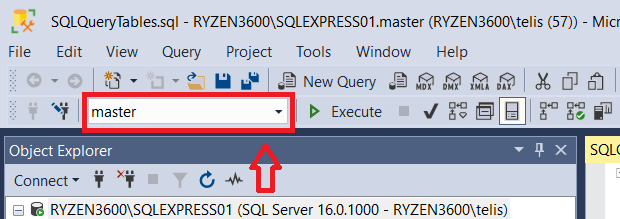
\includegraphics[width=0.65\textwidth]{sqls.png}
		\caption{}
		%\label{fig:emptyView}
	\end{figure}
	
	\item Αποσυμπιέζουμε το αρχείο \textbf{UniversityApp.zip} από τα παραδοτέα το οποίο περιέχει το Visual Studio project.
	
	\item Ανοίγουμε το project μέσω του Visual Studio από το \textbf{.sln} αρχείο
	
	\item Τοποθετούμε το σωστό Connection string της βάσης που δημιουργήθηκε στα αρχεία \textbf{appsettings.json} και \textbf{Models/UniversityDBContext.cs}.
	
\end{enumerate}


Η εφαρμογή είναι έτοιμη για εκτέλεση. Παρακάτω δίνονται ορισμένοι λογαριασμοί με τα credentials τους:

\begin{itemize}
	\item Γραμματέας: Username : aboyda0, Password : Jgx8bp1zRC
	\item Καθηγητής: Username : cbococka, Password : Sc5GIg
	\item Φοιτητής: Username : jibbesonu, Password : pFVJ4ra
\end{itemize}

\section{Πηγές}

\begin{itemize}
	\item Free themes for Bootstrap.\\
	\url{https://bootswatch.com/}
	
	\item Cards - Bootstrap v5.0.\\
	\url{https://getbootstrap.com/docs/5.0/components/card/}
	
	\item Tables - Bootstrap v5.0.\\
	\url{https://getbootstrap.com/docs/5.0/content/tables/}
	
	\item Bootstrap Carousel.\\
	\url{https://getbootstrap.com/docs/5.3/examples/carousel/}
	
	\item Bootstrap Modals.\\
	\url{https://getbootstrap.com/docs/5.3/examples/modals/}
	
	\item Bootstrap Sign-in.\\
	\url{getbootstrap.com/docs/5.3/examples/sign-in/}
\end{itemize}


\end{document}
